% ---------------------------------------------------------------------
% Das Dokument kompiliert mit pdflatex und ist auf Basis 
% von Koma-Script entstanden. 
%
% Autor des Templates (für Anmerkungen): 
% Michael von Riegen, riegen@informatik.uni-hamburg.de
%
% Einzelne Code-Teile für das Titelblatt sind aus dem Template 
% von Benjamin Kirchheim entnommen.
%
% 25.05.09, Frank Langanke: Vorlage auf aktuelle KOMA-Version aktualisiert
% 26.05.09, Michael von Riegen: Anmerkung --> aktuelles Koma-Script ist nötig!
% 17.10.2016 neues Uni logo
% ---------------------------------------------------------------------
\documentclass[11pt,DIV=15,BCOR=20mm,bibliography=totoc]{scrbook}

% Import von Paketen und Optionen die das gesamte Dokument betreffen
% sind in myPreamble.sty ausgelagert.
\usepackage{myPreamble}
   
% Arbeitet man nur an einem Kapitel, wird durch folgenden Befehl nur dieses eingebunden.
% Spart manuelles auskommentieren von vielen include-Befehlen;
% hat keine Auswirkung auf input-Befehle
% \includeonly{kapitel1}
   
\begin{document}


\begin{titlepage}

	% Fehler "destination with the same identifier" unterdrücken...
  \setcounter{page}{-1}

	% Titelseite
	\begin{figure}[h]
		\begin{minipage}[b]{62mm}
			\includegraphics[width=62mm]{images/unilogo}
		\end{minipage}
		\hspace{4cm}
		%\begin{minipage}[b]{59mm}
		%	\includegraphics[width=59mm]{images/minlogo}
		%\end{minipage}
	\end{figure}

	\vfill
	
	\begin{center}
		% Diplomarbeit 
		\noindent { \huge
			Master's Thesis \\
		}
		\vspace{14mm}
		% Titel
		\noindent \textbf{\huge
		Performance-optimized A/B-Testing for E-Commerce-Websites
		}
		\vspace{60mm}	
	\end{center}
	
	\vfill
	
	\noindent \textbf{Aram Yesildeniz} \\
	\noindent \rule{\textwidth}{0.4mm} 
	\noindent{\textrm{max.peter.mustermann@informatik.uni-hamburg.de}} \\
	\noindent{\textrm{Studiengang Informatik}} \\
	\noindent{\textrm{Matr.-Nr. 12345678}} \\
	\begin{tabbing}
	\hspace{8em} \=  \kill
	Erstgutachter: \> Professor A. Ersthelfer \\
	Zweitgutachter: \> Professor Z. Eswirdschonwerden \\
	~ \\
	Abgabe: 01.09.2021
	\end{tabbing}
	
	% Rückseite der Titelseite mit Zitat
	\newpage 
	\thispagestyle{empty}
	\setcounter{page}{0}

	% wenn man Lust auf ein Zitat hat...
	% ... ansonsten auskommentieren
	~\\ \vfill \noindent 
	A distributed system is one where the failure of some \\
	computer I've never heard of can keep me from getting my work done. \\
	\textit{-- Leslie Lamport}
\end{titlepage}





% VERZEICHNISSE (Inhaltsverzeichnis, Abkürzungen)
% Vorspann einleiten --> Seitennummerierung römisch
\frontmatter

% Inhaltsverzeichnis
\tableofcontents
\cleardoublepage


% Hauptteil einleiten --> Seitennummerierung wieder arabisch
\mainmatter



\chapter{Introduction}

[tbd]

\begin{itemize}
	\item Explain structure and main goal of this thesis
	\item Introduction Chapter: Describe shortly all sections from this chapter and what the reader can expect
	\item Give short outlook to following chapter
\end{itemize}


% ---------------------------------------------------------------------------------------------------------
% ---------------------------------------------------------------------------------------------------------


\section{E-Commerce}


% [Internet]
\subsection{The Internet}

In the last 50 years, a new technology emerged, spread over the entire world and influenced many aspect of most peoples life.
Within the turmoil of the cold war, the United State's Advanced Research Projects Agency (ARPA) established in 1957 a communication network to bring together universities and their researches all around the country in order to be able compete against the USSR (\cite{2011Cohen}). % cite 2011 COhen
What started as a tool for scientific collaboration evolved a half century later into the internet, a global network and phenomenon, to which every user with a dedicated device has access and can contribute to.
The internet is an integral part, if not the backbone of today's everyday life.
Users of the internet use it for everything, that is sending emails, watching television, chatting with friends, 
order lunch, checking the weather for the next day or renting motorized scooters.

% [Numbers]

In 2021, the internet has 4.66 billion users, which is around 60\% of the world population.\footnote{Following statistics are taken from \url{https://datareportal.com/reports/digital-2021-germany} [14.05.2021]}
Compared to 2020, the number of internet users increased by 7.3\%.
In Europe, more than 90\% of the population are also internet users.
For a developed country like Germany, the numbers are even more impressing:
94\% of the German population are using the internet with an average daily time of over 5h.

Those numbers demonstrate impressive that the internet is an integral part of our daily life.
Along the rise of internet users, transactions and processes falling under the term of e-commerce rise.
Before discussing the term "e-commerce" and take a grasp at its history and types, some statistics are presented to demonstrate the importance of e-commerce.


% [E-Commerce]
\subsection{E-Commerce}

\subsubsection{Introduction}

From the global data report, we can see that over 90\% of the world population visited an online retail site.
Over 76\% of the world population purchased a product online.
For most categories growth is over 15\%.
Again, for a western country like Germany, the numbers are higher:
92.5\% of the german population visited an online retail site and over 80\% purchased a product online.
And the usage is growing: growth of amount spent in category food and personal care is 28.6\%, and 17.6\% for fashion and beauty.

Revenue in e-commerce is constantly growing over the last 20 years, topping to 57.8 billion in 2019.\footnote{\url{https://einzelhandel.de/presse/zahlenfaktengrafiken/861-online-handel/1889-e-commerce-umsaetze} [14.05.2021]}

% [Corona: Even more growth]

The COVID-19 pandemic with its implications had and still has an not negligible impact on the growth of e-commerce.
Several measures were taken to stop the spread of the virus and the number of deaths, one of which was to minimize physical interaction between people.
This leads consequently to a shift of human interactions to the internet.
Along this, e-commerce benefits.
Bhatti et al. (\cite{2020Bhatti}) conclude that "e-commerce enhanced by COVID-19".

% [E-Commerce History]
\subsubsection{Short History}

E-Commerce, or electronic commerce, is according to the \textit{Encyclopædia Britannica} about "maintaining relationships and conducting business transactions that include selling information, services, and goods by means of computer telecommunications networks."\footnote{\url{https://www.britannica.com/technology/e-commerce} [19.05.2021]}
In short, e-commerce is about buying and selling products and services via the internet.

% TODO check for Tian when paper available:
The success of e-commerce is tightly coupled to the vast advances of internet technology in the past years, like for example the development of the Electronic Data Interchange (EDI) starting from the 1960s, which standardised the communication between two machines.

Personal computers in 1980s and one of the first examples of online shopping is from CompuServe who introduced Electronic Mall in 1984.

Another milestone is Word Wide Web, introduced in 1990 by Tim Berners-Lee, made internet accessible to everyone.
First browser by Tim.

Social media since 2000 again offeres new possibilities for businesses and consumers alike to participate in e-commerce, e.g. for marketing, selling channels

New devices such as smart phones and tablets again decreases the hurdle to participate in e-commerce.
While in the time dimension e-commerce was already available all the time, with the new mobility its also available everywhere.
More flexible.
\cite{2019Hermogeno}.

With the ongoing progress in technology, also e-commerce can expect a shining future with trends such as AI recommendation systems, outstanding UX thanks to Virtual Reality, simple payment methods with crypto etc.\footnote{\url{https://www.spiralytics.com/blog/past-present-future-ecommerce/} [19.05.2021]}


% [Types]
\subsubsection{Types}

Multiple types in e-commerce are existing. They emerge from the possible combinations between the actors \textit{business}, \textit{consumer} and \textit{government} (\cite{2017DosSantos}).

\begin{itemize}
\item B2B: Business to Business
\item B2C: Business to Consumer
\item C2C: Consumer to Consumer
\item G2C: Government to Consumer
\item B2G: Business to Government
\item G2G: Government to Government
\end{itemize}

% [B2C]
\paragraph{B2C}
Business to Consumer in e-commerce describes basically online shopping, by means of a business offering its services and products to the consumer over the World Wide Web.
The consumer can browse within an online shop through the presented products and services and order them directly via the website.
A variety of payment and delivery options conclude the B2C type (\cite{2020Heinemann}).
% cite Heinemann with correct page p. 75 ?

For a aspiring business, multiple ready to use software solutions to install an online shop are existing, for example. Shopify, ePages, Magento or WooCommerce (\cite{2019Steireif}).

% [Amazon]
A famous example of a B2C company is Amazon.
On the 16th of July in 1995, Amazon launched as a website and entered the stock market on the 15th of May 1997 (\cite{2019Stone}). % cite also that this is directly from page p. 47 ?
Amazon is successful, the stock started with a price of X, which is at the time of this writing at Y.\footnote{\url{https://finance.yahoo.com/quote/AMZN?p=AMZN} [19.05.2021]}
Today Amazon employs over 1 million employees\footnote{\url{https://www.statista.com/statistics/234488/number-of-amazon-employees/} [19.05.2021]} and serves the wishes of 200 million paying prime members.\footnote{\url{https://www.statista.com/statistics/829113/number-of-paying-amazon-prime-members/} [20.05.2021]}


% [Pro and Con]
By taking a quick look at the pros and cons of maintaining an online shop, we can see that some of the advantages are that there is no need of a real house to present and sell the products, the virtual shop is available to the consumer at any time and has to closing hours; there is a high potential for the online shop as it is part of growing market; online business is scalable; due to tracking algorithms precise targeting as well as data analysis is possible; to start with an online business, not that much float is needed and there are in general lower costs; it is possible to provide a personalized customer experience; 

Some disadvantages are that the speed of market is rapid, competitors arise everyday everywhere, technology evolves quickly while consumers expectations go high (\cite{2019Hermogeno}, \cite{2020Lang}).


% [Performance of online shop is important]
Another downside is that there is no direct or physical concat with the consumer.
As described above, online shopping takes place in the World Wide Web domain.
Consequently, in person interaction between a buyer and a seller is not possible and the shopping event takes place on a website.
Deriving from this fact, the overall virtual user experience needs to be outstanding in order to stay ahead of competition.
The performance of the online shop is one part of the user experience.

In the next section, I will describe the findings between the correlation between user satisfaction and the performance of the retailers web presence.



% ------------------------------------------


\subsection{User Satisfaction and Performance}

% [User Satisfaction]
The aim of this thesis is not to deep dive into terms and concepts or the non-trivial problem of defining user satisfaction, usability or the like.
Therefore the term user satisfaction is in this context loosely defined as how happy the user is with the website he or she interacts with.\footnote{For a discussion cf. "User satisfaction measurement" in } %cite 2010 Islam

% [Performance]
For this context, performance can be understood as the the speed of an online shop, e.g. how long it takes the page to load, how quickly the user can interact with the page, and how the user perceives the performance of the website.
Later we will see that measuring performance is not that trivial and a lot of ideas and metrics are existing to measure it.


% [SpeedHub]
\subsubsection{SpeedHub}

A plethora of information and studies about the phenomenon of user satisfaction and web site performance is collected at \textit{SpeedHub.org}, a portal by \textit{Baqend} in cooperation with \textit{Google} which provides "the largest systematic study of Mobile Site Speed and the Impact on E-Commerce."\footnote{\url{https://www.speedhub.org/} [21.05.2021]}
On the hub, not only studies and reports are available, but also collections of videos and blog posts.

% [code.talks 2019]
In his presentation at code talks 2019, Felix Gessert summarizes the findings and provides insights to the most relevant aspects and questions of the study so far: %cite 2019 Gessert

% [User Profile and Psychology]
The first observation when tackling the question regarding a correlation between the performance of a system and the user satisfaction, is that the users have to be distinguished which leads to the concept of a \textit{User Profile}: Regarding gender, young woman are the most demanding consumers and buy less on slow pages.
Generally, people between 18 and 24 have higher expectations regarding site speed than their older counterparts.

There are also differences between nations and regions, for example people from Japan have the highest expectations, which for a certainty coheres with the technological progress in this country.
Not only the expectations themselves differ geographically, but also how speed influences the users, for example "speed influences New Yorkers more than Californians."

% cite 
% Think Fast, The 2019 Page Speed Report Stats & Trends for Marketers, Unbounce, 2019
% Brain Food, Speed Matters, Designing for Mobile Performance, Google, 2017


What all users have in common is their human psychology. With respect to performance, researchers generally suggest to keep waiting times under 1000 ms in order to keep the users attention.
% cite
% I. Girgorik, High performance browser networking, O'Reilly Media 2013
% Jakob Nielsen, Usability Engineering, Morgan Kaufmann, 1994

% [Devices]
After considering the user itself, the next step is to investigate the influence of the device in use: Studies show that mobile users are more likely to buy products and services than their colleagues using a desktop computer, where iOS users have generally more expectations regarding site speed.
% cite
% Android vs iOS market share 2019 Q2. DeviceAtlas, 2019.
 
% [Context]
Last but not least is the context and the users condition important, where naturally relaxed and calm users perceive sites faster than stressed users or people that are in a hurry.
Also when on the move, users experience sites slower.
% cite Performance Matters. 9 Key Consumer Insights, Akamai, 2014.


% [Studies]
There are many real world examples and studies existing which prove and demonstrate the importance of site speed with respect to user satisfaction and eventually revenue:
\textit{Amazon} fount out that a decrease of 100 ms in page loading leads to -1\% conversion rates.
If the site loads 100 ms faster, \textit{Walmart} observed that the revenue increases by 1\%.
For \textit{Zalando}, increasing site speed by 100 ms leads to an uplift of 0.7\% revenue per session.
% cite
% Greg Linden. Make Data Useful. Standford Data Mining Class CS345A, 2006.
% Shuhei Kagawa, Jeff Cybulski, David Martin Jones, et al.. Landing Time Matters. Zalando Tech Blog, 2018
% C. Crocker, A. Kulick, B. Ram. Real-User Monitoring at Walmart. SF & SV Web Performance Group, 2012

% [SEO]
Search Engine Optimization is heavily impacted by load speed:
For \textit{Google}, 500 ms slower sites lead to a decrease of 20\% in traffic.
\textit{GQs} traffic increased by 80\% after the page load went down from 7 s to 2 s.
And for \textit{Pinterest}, 40\% faster loads led to 15\% more SEO traffic.
% cite
% Lucia Moses. How GQ Cut Its Webpage Load Time By 80 Percent. Digiday, 2015
% Marissa Mayer, Conference Keynote, Web 2.0, 2006.
% Sam Meder, Vadim Antonov, Jeff Chang. Driving User Growth With Performance Improvements, Pinterest Blog, 2017



% [Engagement & Satisfaction]
Also the user engagement and satisfaction rely heavily on load times:  \textit{Forrester} noted an increase of 60\% for the session length while brining down the load time by 80\%.
\textit{Akamai} monitored that the bounce rate climbed up incredible 103\% when the load time increased by 2 seconds.
And for the \textit{AberdeedGroup}, the customer satisfaction dropped by 16\% at one more second delay in response times.
% cite
% Forrester. The Total Economic Impact Of Accelerated Mobile Pages, 2017.
% Akamai, Akamai Online Retail Performance Report: Milliseconds Are Critical, Akamai Blog, 2017
% The Performance of Web Applications: Customers Are Won or Lost in One Second. Aberdeen Group, 2008.



To summarize, many studies and real world examples prove and demonstrate that faster web sites and online shops cause a better user experience and typically lead to happier customers. 
Concluding in commercial terms, one can say with a certainty that page speed equals money.
\\

In order to properly test the impact of performance on the users, a scientific method is needed.
A/B testing as a controlled experiment is one of them and will be explained in the next section.
After a discussion of A/B Testing, I will move on to the examination of \textit{Web Analytics}, a term which subsumes methods, tools and instruments for businesses to better understand their business and customers.


\subsubsection{A/B Testing}

% 2012 Kessler 17.2  AB Tests ?


% 2016 Kohavi
Controlled experiments such as A/B Testing are not a new tool for scientists and researchers and have been used already in the 1920s. % cite Kohavi 2016
With the rise of the internet in the 1990s, the concept has been adopted to the online domain and is as of today widely used by big companies such as Amazon, Facebook or Google to directly test ideas and hypothesises on a live system.
Controlled experiments such as A/B Testing are utilised to support decision making and to deliver "causal relationship with high probability". % cite Kohavi 2016
They enable a data driven and quantitative validation of the hypothesis. % cite Morys 2018

Controlled experiments help to test hypothesis and questions of the form: "If I change feature X, will it help to improve the key performance indicator Y?"

To answer this question,  two systems are needed: Version A, the control variant or default version, and a slightly different version B, called the treatment.
If more than two versions or one treatment should be evaluated at the same time,  an A/B/n split test has to be implemented.
For an univariable setup, only one variable differs between the systems, where in a multivariable structure, more than one variables are changed at the same time.

Usually, the users of the system are randomly split into two groups and testing is directly performed with real users on a production system.
Beneficial, also when comparing with other experimental setups, is, that the users and participants are not aware that they are part of an experiment, which leads to less bias and side effects.
In order to measure the differences and the user behaviour, web analytics has to be integrated within the system.
% cite Kohavi 2016


% TODO write those steps down ?
% 2018 Morys
%- 5 steps:
%- 1. quality of hypothesis according to SOR Paradigma
%- 2. quality of testconcept: isolation and contrast of changed parameters
%- 3. quality of implementation and quality assurance: running tests should not be visible by user (e.g. suddenly UI changes) and performance of website should not be impacted
%- 4. quality of measurement: significant difference in primary goals
%- 5. quality of statistical interpretation: amount of data, statistical methods


A short and general discussion about controlled experiments in computer science is in chapter X. %link chapter about controlled experiments


% [Transition to Web Analytics]

To resume with the question of performance and user satisfaction,  A/B testing enables to serve two different versions of the same site to two groups, one site being slow, the other one fast, at the same time without the users knowing.
With web analytics implemented, it is possible to measure how the different systems and user groups behave.

What web analytics exactly is, what tools are available and how a web analytics process looks like, will be discussed in the next section.




% Heinemann 2020 A/B Tests nach 4.1.4



% ------------------------------------------------------------------------------------
% ------------------------------------------------------------------------------------
% ------------------------------------------------------------------------------------
% ------------------------------------------------------------------------------------




\section{Web Analytics}

First some definitions, then quickly summarize the history, and then technical aspects of collecting data.


\subsection{Introduction}

% [Definitions]
What is Web Analytics?
Going through the literature, makes it clear that multiple definitions are existing:

Nakatani et al. state that "Web analytics is used to understand online customers and their behaviors, design actions influential to them, and ultimately foster behaviors beneficial to the business and achieve the organization's goal." % cite 2011 Nakatani
According to this definition, web analytics is about getting insights of the users using the system, not only who or what they are, but also how they interact with the system.
Additionally, the definition stressed that the underlying motivation of web analytics is are the achievement business goals.

Singal et al provide a more technical definition by pointing out that "Web Analytics is the objective tracking, collection, measurement, reporting and analysis of quantitative internet data to optimize websites and web marketing initiatives." % cite 2014 Singal with note that this definition is directly taken from Kaushik
Again, the ultimate target is to drive business forward, but backed up with data science methods and instruments such as tracking, collecting and analysis of vast amount of data.

Bekavac et al provide a similar definition by pointing out that web analytics is "the analysis of qualitative and quantitative data on the website in order to continuously improve the online experience of visitors, which leads to more efficient and effective realization of the company's planned goals." %cite 2015 Bekavac:

% TODO: where can i find this officially ?
% Official definition by WAA: the measurement, collection, analysis and reporting of Internet data for the purposes of understanding and optimizing Web usage.

% TODO add 2009 Waisberg? "Web Analytics can be defined as the act of increasing a website’s persuasion and relevancy to achieve higher conversion rates."

% TODO add Croll 2009? "Today, web analytics is a marketing discipline used to measure the effectiveness of communications strategies" p.83

Summarizing above definitions, we can see that web analytics is composed of two important aspects: A data driven, information focused and technical aspect of collecting and analysis data about the users, and a commercial perspective, which provides the main motivation of collecting the data beforehand, by setting business goals.


% [Use Cases]
Moving from the definitions to the practical domain, Zheng et al. describe four main use cases for web analytics:

% 2015 Zheng
% TODO write more here
\begin{itemize}
\item Improve overall design and user experience
\item Optimize for your business goals
\item Monitoring
\item Improve performance
\end{itemize}

Those use cases in the end also target to make customers more happy and increase revenue.


% [Challenges]
Web analytics is also difficult and there are some obstacles to avoid and challenges to tackle.

% 2019 Kumar
Kumar et al. describe the hurdles as follows:
Data science challenges:
Statistical methods are not yet sophisticated enough.
Collected data is heterogeneous and incomplete.
A lot of data is available (big data).
Analysis not fast enough.

Privacy: tbd




% ------------------------------------------


\subsection{Short History}

The history of web analytics can be described as its shift from an IT domain and technical log file analysis tool towards a sophisticated, polymorphic instrument for marketers.

% [For IT: Logs]
% TODO add somewhere: Log file analysis is discussed in greater detail in chapter X. %refernece chapter

Everytime a user requests an html file or another resource from the webserver, an entry in a dedicated log file is made by the server. %cite Singal 2014
The first log entries followed the Common Log Format (CLF) which provides rudimentary information such as the date, the HTTP status code or the number of bytes transmitted.
In 1996, the Extended Log Format (ELF) was introduced with more flexibility and information in mind.
Thanks to the standardized format of log files, software could be build to analyse the log files and present them in a user friendly fashion.
\textit{GetStats} was one of the first tools which generated statistics and user friendly output for analysts.
% cite Croll 2009 p 69
and in 1995, Dr. Stephen Turner created Analog, the first free log file analysis software.% cite Zheng 2015

% [Shift]

What was in the beginning mainly interesting for maintenance and IT personal who answered questions such as how many 404s occurred on the server, turned into a website information pool interesting for marketers.

With the increase in available information it came clear that the data can be used for more than just analysing the servers behaviour.
But log file analysis was not sufficient enough to get details about how users interact with the website.
Web analytics experienced a transformation from log analysis logging to user data tracking, analysis and reporting.

Croll describes the move of analytics from IT to marketing with three steps: %cite Croll 2009
\begin{enumerate}
\item JavaScript made log files redundant and also empowered marketers to maintain and implement their analytics solutions, unravelling their dependence from the IT department.
\item The introduced advertisement economy from search engines like Google led to a new focus for analysts on user attraction and conversion rates.
\item New cost models enabled the marketers to pay for the analytics service according to the websites traffic, instead of paying for hard- and software in advance. The expenses for analytics were therefore coupled with the websites traffic and ideally revenue.
\end{enumerate}


% [For Marketing: JS]

In 1990 the \textit{World Wide Web} kicked off and one of the first widely used browsers \textit{Mosaic} launched in 1993.
At the same time \textit{WebTrends} developed and released one of the first analytics software.
A lot more services followed, such as \textit{WebSideStory} in 1996 % cite Zheng 2015
or Quantified by Urchin in the same year.%cite croll 2009

The page tagging technique enabled the collection of not only technical data, but also business relevant information.
Visitors and their behaviour were the main concern and coined to questions such as: How is this user behaviour linked to a purchase? If a user buys shoes, will he also buy socks?
The development and implementation of Cookies enabled the identification of unique users.
Not only business related questions were asked and answered, but also investigations of performance and usability.
% cite 2009 Croll p. 69

More details about page tagging in chapter X.


% 2014 Singal
In 2003, Edwards, Eisenberg and Sterne founded the Web Analytics Association (WAA).
The WAA is brings together and supports all actors of web analytics such as users, marketers and IT specialists on an international stage.
Due to the digitalization and its all-embracing impact, WAA renamed itself to Digital Analytics Association (DAA), as the web is not the only domain where users leave their digital footprint.
% cite 2014 Singal

As already described in the above section, the numbers of participants and users of the internet are still increasing and all Fortune 500 companies operate websites, with Web Analytics as a centrepiece tool in marketing. %cite Kumar 2019

Some of the most established tools today are Google Analytics, Adobe SiteCatalyst, Webtrekk and Piwik. % cite Heinemann 2020 4.1.4

Google Analyitcs will be discussed in chapter X.

Zheng et al. identify several future trends for Web Analytics, such as mobile web and application specific analytics like video-, search-, learning- or social media analytics. %cite Zheng 2015


% TODO add Image: Genesis of Web Analytics (nice graphic) with WAA, DAA ? should remove then in-page analytics arrow
% TODO add somewhere Some methods about tool selection are described in chapter X.

% TODO next section will be about process


% ------------------------------------------



\subsection{Web Analytics Process}


Web Analytics can be described as a process, where as a rule the main goal is to increase revenue.
In literature, two main ideas and process flows are indicated, the first one being from the Web Analytics Association, and the second one derived from industries best practices.
They will be concisely described in this section.

What both processes have in common is that they aim for improving the website and consequently increase the business revenue.

\textit{Key Performance Indicators} (KPIs) are the ideal tool to instrument web analytics and they help to determine areas and room for improving.
They are an integral part and play a major role in any web analytics process as they provide an "in-depth picture of visitor behavior on a site". %cite 2009 Jansen ch. 6.2

KPIs can differ according to the business they operate it.
For commercial domains, common KPIs are conversion rates, average order or visit value, customer loyalty, bounce rate, and so on.% cite 2014 Singal
Defining the right KPIs and align them with the business goals is a crucial step in any web analytics process.

% 2015 Bekavac:  KPIs for commercial model: Ratio of new to returning visitors, percentage of new visitors, referring domains, search keywords/phrases, average order value, key conversion rates



\subsubsection{WAA Process Guide}

Web Analytics Association provides a nine step guide:% cite 2009 Jansen ch. 6.2
\begin{enumerate}
\item Identify key stake holders
\item define primary goals of website and prioritize them
\item identify most important site visitors
\item determine key performance indicators
\item Identify and Implement the Right Solution
\item Use Multiple Technologies and Methods
\item Make Improvements Iteratively
\item Hire and Empower a Full-Time Analyst
\item Establish a Process of Continuous Improvement
\end{enumerate}



\subsubsection{Industries Best Practices}

Waisberg and Kaushik derive from industries best practices a five step process with the main goal, improve website, increase revenue, in mind:% cite 2009 Waisberg

\begin{itemize}
\item Define Goals
\item Build KPIs
\item Collect Data
\item Analyze Data
\item Implement Changes
\item Repeat last two steps
\end{itemize}
% TODO add graphic instead of list


% [Comparison]
Comparing both proposed processes, it is evident that both put the identification and awareness of the main business goals upfront.
WAAs process is are more fine grained and practical approach, where as Waisberg and Kaushiks flow abstracts the principal activities.


% ------------------------------------------



\subsection{Data Collection/Sources: Log Analysis versus Page tagging}

There are four main ways to collect data for web analytics: Logs, JavaScript Tagging (or page tagging), web beacons and packet sniffing. %cite 2009 Waisberg

As already mentioned in chapter X,  the two main data collection methods are Log file analysis and Page Tagging.
In this section, I will briefly describe both mechanisms and compare them to each other.


\subsubsection{Log File Analysis}

As already described in the above section X, log file analysis is about getting insights from the web servers log files records.

Log file analysis is considered to be the traditional and original approach to web analytics. %cite 2011 Marek and 2015 Zheng

Once the users enters a URL in the browser and hits enter, the request arrives at some web server.
The server then creates an entry in a log file and sends back the requested page or resource as a response to the client. % cite % 2009 Waisberg

The information within the log entry can vary depending on the log format, mostly provided are the IP, browser, timestamp, time taken, bytes transferred, whether a cache hit occured and the referrer. %cite 2009 Waisberg

The standardized Common Log Format provides host, ident, authuser, date, request, status, bytes, as seen in example X. \footnote{\url{https://www.w3.org/Daemon/User/Config/Logging.html\#common-logfile-format} [03.06.2021]}

\begin{center}
\begin{lstlisting}[caption={Position 1}, language=bash, numbers=none, basicstyle=\tiny]
127.0.0.1 user-identifier frank [10/Oct/2000:13:55:36 -0700] "GET /apache_pb.gif HTTP/1.0" 200 2326
\end{lstlisting}
\end{center}
% TODO add caption

Standard formats of log files and entries allow log file analysis software to process, evaluate and report valuable statistics to users, such as Analog, Webalizer or AWStats. %cite 2015 Zheng


% [Pro]
Following are lists describing the advantages and disadvantages of log file analysis.

Advantages of log file analysis are:

\begin{itemize}
\item JavaScript and Cookies are not required on the client side
\item Maintainer of the website and server owns the data %cite 2009 Waisberg
\item Bots and web crawler requests are also logged %cite 2009 Waisberg
\item History of data is available %cite 2011 Nakatani
\item Log entries are reliable %cite 2011 Nakatani
\item The standard format of log files enables easy switching of analysis tools %cite 2011 Nakatani
\item The web server also logs failed requests %cite 2011 Nakatani
\item No modification on the web page needed %cite 2015 Zheng
\item Does not demand more bandwidth %cite 2014 Singal
\end{itemize}


% [Con]
Some disadvantages are:

\begin{itemize}
\item Log entries provide mainly technical information, which may not be very useful for user behaviour analysis. Business related metrics such as bounce rates are not available. % cite Marek 2011
\item Only direct requests from the client to the web server are logged: Any user interaction in the web browser, which does not fires a request, is not getting logged. Also responses from caches and proxies are not visible in the web servers log file. Only interactions with the web server are logged.%cite 2015 Zheng
\end{itemize}



% ------------------------------------------


\subsubsection{Page Tagging}

In a nutshell, page tagging describes the analytics method of including JavaScript on the web page, which collects data and sends it to an analytics server. %cite 2011 Marek
For this, JavaScript has to be included on every page which should be analysed. %cite 2009 Waisberg
Page tagging is the main method used in web analytics today. %cite 2015 Zheng

Croll provides a vivid graphic about the page tagging process which will be discussed here (fig. X). %cite Croll 2009

\begin{center}
\includegraphics[width=0.5\textwidth]{page_tagging.png}
% TODO add caption
\end{center}

The client (browser) requests a page from the web server (1, 2).
Within the html file an external JavaScript resource, the analytics code, is linked and received from the analytics server (3, 4).
The analytics script tracks and measures the user behaviour and eventually sends the data back to the analytics server (5, 6, 7).

The collected data can also be stored in cookies, which persist data beyond one session and enable user identification, e.g. on his next page visit. %cite 2019 Kumar


The advantages and disadvantages of page tagging are as follows:

% [Pro]
\begin{itemize}
\item Every page visit is counted %cite 2009 Waisberg
\item The analytics service is outsourced, which includes the storage of the data, but also data analysis and reporting %cite 2009 Waisberg
\item Page tagging is rather easy to implement and favourable when the analyst does not have access to the web server %cite 2011 Marek
\item Highly customizable: anything that JavaScript allows to measure, collect and track is obtainable. This also includes information about the client such as screen size, device used or color depth. %cite 2011 Nakatani
\item Possibility to track events and actions such as mouse clicks that do not send requests to the web server. This is especially important for single-page or progressive web applications which do not fire requests that often. %cite 2011 Nakatani and 2015 Zheng
\item Mechanics of cookies provide identification of unique and repeat visitors %cite 2011 Nakatani
\item Real time reporting %cite  2014 Singal 
\end{itemize}



% [Con]
Some disadvantages are mainly privacy concerns, the analytics process relies on the usage of JavaScript and cookies which can be deactivated by the user %cite 2011 Marek
, every page which should collect data needs to include the analytics script, and due to the use of a third party analytics service it is rather difficult to switch tools. %cite 2014 Singal


% TODO 2017 Hassler ch. 2 ??

% TODO web beacons and packet sniffig ?
% 2011 Marek
% 2011 Nakatani
% 2014 Singal




% ------------------------------------------






\subsection{Web Performance}

\begin{itemize}
\item What is web performance? Why it matters
\item Overview of factors that impact performance, bottlenecks
\item Overview of measurement methods, techniques and metrics
\end{itemize}

% very short introduction about performance:
% - bottlenecks
% - why bother with performance ? we already saw this with the studies
% SEO

% this is introduction chapter, so refer here to other chapters where topics are covered in detail
% Metrics
% Measurung methods and tools; synthetic vs rum
% Link here to other chapters:
Metrics in chapter X
Measuring methods in chapter Y
Practical example and experiment in chapter Z



% Bottlenecks of performance, big picture:
% 2013 Grigorik: Latency as bottleneck and not bandwith


% 2016 Witt




Measure performance:
% 2021 Wolle blog post https://medium.baqend.com/mobile-site-speed-measurement-best-practices-ff4a3f91b003
- Log file
- Synthetic
- RUM
- CrUX
- Surveys


% 2016 Kaur: Tools for Measuring the Performance of Websites


% https://developer.mozilla.org/en-US/docs/Learn/Performance/What_is_web_performance
- notes





% https://developer.mozilla.org/en-US/docs/Learn/Performance/Measuring_performance
- notes




% ------------------------------------------------------------------------------------
% ------------------------------------------------------------------------------------
% ------------------------------------------------------------------------------------
% ------------------------------------------------------------------------------------




\section{Research Question}

\begin{itemize}
\item Difficulty of defining scope
\item Measuring performance of a web site impacts its performance or other effects take place / Observer effect
\item Why the research question is relevant
\end{itemize}

What is the research question of this thesis?
What is the goal?

the intrinsic complexity of the field and the internet in general

% Measuring Real User Performance in the Browser: Avoiding the Observer Effect



Motivation


Goals of this thesis


\subsection{Chapter Outline}

This introduction chapter was about

In chapter X...

tbd













% Terms and Definitions
%TODO maybe move stuff from chapter 1 in this chapter
\chapter{Metrics and Measurement Methods}

[tbd]

\begin{itemize}
	\item Last chapter...
	\item This chapter: In this chapter, I will cover measurement methods and discuss common performance metrics.
	\begin{itemize}
		\item This chapter should cover all relevant terms and definitions within web performance measurement
		\item How terms can be structured / taxonomy
		\item Ambiguity of definitions
	\end{itemize}
	\item In the next chapter...
\end{itemize}


- Technical Background:
	- Network
	- Front End: Navigation and CRP
	
- Metrics

- Measuring Methods



% https://developer.mozilla.org/en-US/docs/Learn/Performance/Measuring_performance
- Compare to competitors
- Compare different versions of your app
- Metrics should be relevant to your users, site, and business goals
- should be collected and measured in a consistent manner
- analyzed in a format that can be consumed and understood by non-technical stakeholders



% 2004 Phippen



% TODO
% IF possible use more cool tables


% ---------------------------------------------------------------------------------------------------
% ---------------------------------------------------------------------------------------------------


%TODO find better title
\section{How Websites are being loaded}

% [Introduction]
- Brief technical introduction
- It is important to understand how things work, because Metrics and also how to measure them are derived from those processes

In order to understand web performance metrics and the methods to measure them, it is crucial to have a basic understanding of the technical aspect of loading a website into a browser.
This process includes establishing a connection between a client and a server, which will be discussed in section X, and the task of the browser to transform the received data from the server into a readable ready-to-use website, which will be discussed in section X.
Always with performance in mind.

% [3 Entities: FE, BE, Network]
It is possible to divide the website loading process into three entities which play a role.
In his code talk 2016, Witt identifies three main areas or bottlenecks where bad performance is being produced: In the Frontend, the Backend, and on the network layer.  % cite 2016 Witt or just say this ??
The Front End is everyhting the user sees on the screen, client, UI, browser, sends requests to a back end, etc.
The Back End is the logic, servier, also data base, handles requests and sends responses to a front end
Network is what connects clients and servers, FE and BE, infrastructure element composed of routers, cables, wireless connections etc.


- BE is not discussed (server time, data base, etc.)
- Section X is about Network
- Section X is about Front end: how browser works, crp, 
- How to optimise websites is not part of this thesis

In this section, i will also say which metrics are describing the underlying process.
So this section links directly to the metrics section.
But all metrics are collected in the metrics section.



% --------------------------------------------------------------------------------------------
% --------------------------------------------------------------------------------------------


%TODO choose title. Maybe "Establishment of Connection?"
\subsection{The Network Realm}

Starting from hardware, ISP, routers, switches etc and the cables connecting them is part of the network.
But also communication protocols such as the Internet protocol suite.

Regarding performance, latency and bandwidth come into mind, and we will see that latency has a bigger impact on performance than bandwidth in section X.

After discussing this issue, i will continue by describing the process or navigation steps which happen once the user enters a URL into the browser, up until he sees pixels on his screen and can use the website.


% --------------------------------------------------------------------------------------------


\subsubsection{Latency and Bandwidth}

There are two important attributes when discussing network performance: Latency and Bandwidth.
The important thing to say here is that Latency is bottleneck for performance, and not bandwidth.


% [Bandwidth]

Bandwidth is the "maximum throughput of a logical or physical communication path". %cite 2013 Grigorik
In other words, bandwidth describes the amount of data which can be sent in parallel from one node in a network to another. 

Physical communication paths are most likely cables such as metal wires or fiber-optic cables, where fiber-optic cables have less signal loss, and lower lifetime maintenance costs.
With methods such as wavelength-division multiplexing (WDM), it is possible to transmit up to 70 Tbit/s over a fiber-optic connection.  %cite 2013 Grigorik

This high technology stuff is only used in the backbone infrastructure, e.g. for connecting Europe with America.
For the end user, bandwidth is much lower, and the average was in late 2015 just 5.1 Mbps %cite 2013 Grigorik

A high bandwidth is useful for bulk or large data transfer such as streaming of video or audio.
But for loading a website,or any browser activity that depends on many requests that fetch data from many different locations around the globe, the performance bottleneck is latency. % cite 2013 Grigorik


% [Latency]

Latency is "the time from the source sending a packet to the destination receiving it".  % cite 2013 Grigorik

Latency is measured in seconds and can be the time spent for one-way, or more common, how long it takes for the transmitted data package for the round-trip time (RTT), from source to destination and back.
In other words, latency "describes the amount of delay on a network or Internet connection". % cite https://developer.mozilla.org/en-US/docs/Web/Performance/Understanding_latency

For the very first request when establishing a connection, latency is longer due to protocols such as DNS lookup, TCP and TLS handshakes.
Those will be discussed in section X. % cite https://developer.mozilla.org/en-US/docs/Web/Performance/Understanding_latency


% [Experiment]

To get an idea about how the two aspects, bandwidth and latency, impact web performance,  Mike Belshe launched a study. % cite https://docs.google.com/a/chromium.org/viewer?a=v&pid=sites&srcid=Y2hyb21pdW0ub3JnfGRldnxneDoxMzcyOWI1N2I4YzI3NzE2
Once setup has a fixed latency and bandwidth is variable, and vice versa.
He and compared the performance of the two experiments using the Page Load Time metric. (cf. X for this metric)


\begin{figure}[h!]
\begin{center}
\includegraphics[width=0.8\textwidth]{latency.png}
\caption{Latency vs Bandwidth}
\label{img:latency}
\end{center}
\end{figure}


We can see that the impact of bandwidth is trivial: if the available bandwidth is doubled, e.g. from 5 to 10 Mbps, there is no change in performance load time.
For Latency on the other hand, the picture is different: If the latency can be decreased by half, e.g. from 120 ms to 60 ms, the page load time also sinkt um die hälfte.

Or as Belshe states it, "[reducing] cross-atlantic RTTs from 150ms to 100ms [...] would have a larger effect on the speed of the internet than increasing a user's bandwidth from 3.9Mbps to 10Mbps or even 1Gbps." % cite https://docs.google.com/a/chromium.org/viewer?a=v&pid=sites&srcid=Y2hyb21pdW0ub3JnfGRldnxneDoxMzcyOWI1N2I4YzI3NzE2

This obersvations can be explained with the many short, small connections and requests are made when browsing websites and the contrary underlying structure of the communication protocols, which are "optimized for long-lived connections and bulk data transfers. " %cite 2013 Grigorik ch 10

But just simply decreasing the latency is not straightforward: The speed of data transfer is already at a 2/3 of light, but the physical constraint is the limiting factor, e.g. there is a minimum distance between London and New York which can not be further "optimized". % cite 2013 Grigorik Ch 1


% [Mobile]

Another aspect of latency is that for wireless connections and therefore mobile devices, latency is even higher, "making networking optimization a critical priority for the mobile web." % cite 2013 Grigork Ch 1

This is due to the infrastructure of mobile nets, latency is high for mobile users. cf.  Why are mobile latencies so high? in Grigorik % cite https://www.igvita.com/slides/2013/fluent-perfcourse.pdf


% [Transition]

As latency is a important factor, what happens on the front end is still important.
And again for this thesis metrics measuring performance in the front end are the focus.

Before i will discuss what happens in the browser once the website data arrived, i will briefly describe the preceding steps of establishing a connection between the browser (client) and the server.



%TODO add this ?

% Use other techniques such as CDNs, caching, pre-fetching, etc % 2013 Grigorik
% CDN: Help against this issue. Put stuff close to client % 2013 Grigorik

% Some direct implications for performance measurement ?
% Understanding Latency https://developer.mozilla.org/en-US/docs/Web/Performance/Understanding_latency
% Network throttling: Emulate download speed, upload speed, and minimum latency



% --------------------------------------------------------------------------------------------



\subsubsection{Navigation Process}

I will explain briefly the general navigation process: It begins when the user is submitting a URL in the browser and ends when he received website data.

The main steps can be divided into networking, that is, establishing a connection with DNS etc., backend processing, e.g. data base queries etc., and the rendering in the front end, as seen in image X.
The last part of this process is when browser receives finally the HTML / Document. 
How the browser transfers the HTML into an interactive website is part of the next section.


"To start, it is important to recognize that every HTTP request is composed of a number of separate stages (Figure 10-3): DNS resolution, TCP connection handshake, TLS negotiation (if required), dispatch of the HTTP request, followed by content download." % cite Grigorik 2013


\begin{figure}[h!]
\begin{center}
\includegraphics[width=0.8\textwidth]{timing_overview.png}
\caption{Timing Overview}
\label{img:timing_overview}
\end{center}
\end{figure}
%TODO change image: remove network and BE boxes? remove white space around image


%TODO add this ?
% Understanding Latency https://developer.mozilla.org/en-US/docs/Web/Performance/Understanding_latency
%Network Timings:
%- Blocked: When a request is in queue
%- Blocking happens when there are too many simultaneous connections to single server over HTTP



% ----------------------------------


\paragraph{DNS Lookup}

When the requested resource can not be loaded from the browsers cache, the first step to establish a connection is a DNS Lookup (or DNS Resolution).

This step is about translate URL to IP address.
Must be done for each unknown URL, e.g. when linked images within a website are from different server, for each unique URL DNS Lookup has to be done.
The mapping of URL to IP can be cached by browser, which makes repeated views faster. % cite https://developer.mozilla.org/en-US/docs/Web/Performance/How_browsers_work

Avg. time is 20 and 120 ms % https://www.keycdn.com/support/reduce-dns-lookups
Can be considered a performance metric, see section X.


% ----------------------------------


\paragraph{TCP Handshake}

Once a connection between a client and a server is established, the TCP 3-way-Handshake comes into play.

The goal of TCP is to establish a reliable connection within an unreliable network.
TCP  "guaranteed that all bytes sent will be identical with bytes received and that they will arrive in the same order to the client. " %cite 2013 Grigorik
Regarding performance, the handshake adds two more round trips, which is bad for performance as we have seen because of latency.

Many algorithms and techniques to get optimal data transfer and also avoid congestion are existing, such as Slow-Start.
Slow-Start is an algorithm that determines the maximum bandwidth that can be used by gradually increasing the amount of data sent.
Slow start prevents that the full capacity of the network is being used from the beginning, which in performance terms adds again more round trips and latency. %cite 2013 Grigorik


%TODO once i know which metric add it here
A performance metric reflecting the time spent for establishing a TCP connection is X, see section X.
For a detailed discussion cf "Building Blocks of TCP" in 2013 Grigorik % cite https://hpbn.co/building-blocks-of-tcp/


% ----------------------------------


\paragraph{TLS Negotiation}

TLS is another protocol which has the goal to establish a secure connection in terms of data encryption.
Data transmitted over the network has to be encrypted so that aussenstehende can not read or manipulate the data.
For encryption,  a cipher to be used needs to be established, which will be shared between client and server during the TLS Negotiation. % cite https://developer.mozilla.org/en-US/docs/Web/Performance/How_browsers_work

TLS again adds more round trips which is bad for performance.

%TODO once i know which metric add it here
A performance metric reflecting the time spent for a TLS negotiating is blabla in section X.

for a detailed discussion see Transport Layer Security (TLS) in 2013 Grigorik % https://hpbn.co/transport-layer-security-tls/


% ----------------------------------


\paragraph{HTTP Request and Response}

Now that a secure connection is established, the client fetches the first resources via HTTP GET request.
Most often, the server will respond by sending back the index.html file, which then can be used by the browser to build the website. % cite https://developer.mozilla.org/en-US/docs/Web/Performance/How_browsers_work

The time when this first response containing the first byte for building the web site is reflected in the metric TTFB which is discussed in section X.


% [Connection vs Request]

Usually, many more resources are requested by the browser to complete the build of the web site.
As of today, the median value is about 70 requests per web site. % footnote https://httparchive.org/reports/state-of-the-web#reqTotal

A request is not the same as a connection.
Once the connection is established via the above described procedures such as DNS lookup, TCP and TLS handshakes, multiple requests can be transmitted over the same connection.
Usually, the number of requests is much higher than the number of connections to load a website, as the browser persist connections, keep them open for multiple requests.
Median connections for a web site today is about 13. % footnoe https://httparchive.org/reports/state-of-the-web#tcp
Modern browsers like Chrome enable up to six open connections in parallel. % cite 2014 Hogan



% [Transition to CRP]

At this point, the browser has received the first data about the web site and he can start with rendering the page.
How this exactly happens, is explained in the next section.




% --------------------------------------------------------------------------------------------
% --------------------------------------------------------------------------------------------



\subsection{Front End: Critical Rendering Path}

This section explains what happens after the first bytes of the web sites arrived in the browser.
The following processes are typically subsumed under the term \textit{Critical Rendering Path} (CRP).
The CRP is the last part of the navigation process as seen in image X.


% [Critical]

The CRP is the minimum steps that the browser has to take from the moment it receives the first byte of HTML to the moment that it renders pixels on the screen for the first time.

The rendering is critical as it is the very first render, the first visible content the user will see on the screen.
The resources that are needed for the first render of the page delay the first render of the page are considered to be critical.
Without the critical resources, the browser can not display content on the screen.
An example of a critical resource is the first HTML file the browser receives, as without it, nothing is visible on the screen.
Non-critical resources on the other hand will not stop the browser from displaying the first content on the screen. % cite https://blog.logrocket.com/how-css-works-parsing-painting-css-in-the-critical-rendering-path-b3ee290762d3/


% https://gtmetrix.com/blog/how-to-eliminate-render-blocking-resources/
%- Non-critical resources are those that provide contributions to secondary/tertiary functionality or styling for the content on your page, e.g., a calendar widget on the sidebar below-the-fold.


% https://blog.logrocket.com/how-css-works-parsing-painting-css-in-the-critical-rendering-path-b3ee290762d3/
%- Any CSS that is not necessary for the first load can be considered “non-critical”



% [CRP Steps]

There are a sequence of steps the browser goes through to render the page.
The basic idea is to convert HTML, CSS and JS to actual pixels on the screen.

Image X visualizes the flow of the CRP:
Once the HTML is received, the browser starts with parsing the HTML and translate it into the DOM.
The content of the CSS files will be parsed to the CSSOM.
JavaScript needs to be fetched and executed.
Once DOM and CSSOM are available, the Render Tree is being created.
When the Render Tree is available, Layout is happening.
Finally, pixels can be printed on the screen.
% cite https://developer.mozilla.org/en-US/docs/Web/Performance/Critical_rendering_path

In the following, the individual steps will be discussed in more detail.


\begin{figure}[h!]
\begin{center}
\includegraphics[width=0.7\textwidth]{crp.png}
\caption{Critical Rendering Path}
\label{img:crp}
\end{center}
\end{figure}




% [Single Thread]
%TODO do i need this ?
% How Browsers Work https://developer.mozilla.org/en-US/docs/Web/Performance/How_browsers_work
%- This is somewhat the bottleneck or the technical state of the browser
%- Browser is single threaded
%- Still: Enable smooth interaction: scrolling, responsive to touch, etc.
%- Render time is key
%- Goal: Main thread can complete all the work and still is available to handle user interaction
%-> Improvement: Understand single thread concept of browser and minimize main threads responsibilities
%-> Should lead to: rendering is fast and smooth and responses to interactions are immediate



\begin{figure}[h!]
\begin{center}
\includegraphics[width=0.7\textwidth]{crp.png}
\caption{Critical Rendering Path}
\label{img:crp}
\end{center}
\end{figure}


\paragraph{DOM Construction from HTML}

% [Introduction, Standard]

Once the browser received the first bytes of the HTML file, it starts to parse it into the \textit{Document Object Model} (DOM).
The DOM construction is the first step the browser performs when receiving data.
The DOM is a tree structure and internal representation of the HTML for the browser. % cite https://developer.mozilla.org/en-US/docs/Web/Performance/How_browsers_work
The general parsing process consists of translating from bytes to characters, to tokens, to nodes and finally to the object model.% cite https://developers.google.com/web/fundamentals/performance/critical-rendering-path/constructing-the-object-model
The specification of the DOM is maintained by the WHATWG living standard. % footnote https://dom.spec.whatwg.org/

% The Parsing of the HTML into the DOM is defined in the HTML standard % footnote https://html.spec.whatwg.org/multipage/parsing.html#parsing


% [Render Blocking]

The DOM tree contains information about the content of the document, but not its style.
The styling is defined in the CSS.
Once HTML and CSS are transmitted and processed by the browser, the \textit{Render Tree} can be created, which reflects the actual information and its styling the browser can display.
Within this context, it is possible to categorise resources into render blocking and non-render blocking.
A render blocking resource is a resource that prevents the browser from rendering content to the screen.
HTML and CSS are render blocking resources, as the parsing process of those files blocks the browser of displaying the page to the screen.% cite https://developers.google.com/web/fundamentals/performance/critical-rendering-path/render-blocking-css

% CSS parsing and render tree construction will be discussed below.


% [Incrementally]

As soon as the first data packages of HTML arrive at the browser, the parsing process starts. %cite How Browsers Work https://developer.mozilla.org/en-US/docs/Web/Performance/How_browsers_work
The DOM is created incrementally,  this means that the browser can begin to process the HTML before all of its content is transmitted over the network.


% [Resources]

Usually, within the HTML, external resources are linked which are necessary for the website to be complete, such as CSS or JavaScript.
While parsing the HTML incrementally, eventually a reference to such an external resource will be encountered.
How the external resources CSS and JavaScript are being handled by the browser is discussed below.


%TODO add this?

% How Browsers Work https://developer.mozilla.org/en-US/docs/Web/Performance/How_browsers_work
%- DOM is also exposed, and can be manipulated through various APIs in JavaScript 
%Optimisation: Preload scanner:
%- This process occupies main thread while browser is building DOM Tree
%- parse through the content available and request high priority resources like CSS, JavaScript, and web fonts.
%- will retrieve resources in the background so that by the time the main HTML parser reaches requested assets, they may possibly already be in flight, or have been downloaded




% ------------------------------------------------------------


\paragraph{CSSOM Construction from CSS}


% [Introduction]

The CSS resource contains all information about the styling of the page.
As with the HTML,CSS is converted from bytes to characters, to tokens, to nodes, and finally to the \textit{CSS Object Model} (CSSOM). % cite https://developers.google.com/web/fundamentals/performance/critical-rendering-path/constructing-the-object-model
CSSOM construction is usually very fast . % cite % How Browsers Work https://developer.mozilla.org/en-US/docs/Web/Performance/How_browsers_work
CSSOM is standardized here % footnote https://drafts.csswg.org/cssom/

% The DOM and and CSSOM are separated structures and not yet connected.
% The Render Tree reflects the combination of the two models and will be discussed below.
% Creation of CSSOM happens after DOM is completed. % https://developer.mozilla.org/en-US/docs/Web/Performance/Critical_rendering_path



% [Cascading, Not incrementally]

As opposed to the HTML parsing process, CSS can not be translated to the CSSOM incrementally.
Cause it the cascading nature of style sheets, which has the potential that the styling rules defined at the top of the file may be overridden by rules defined at the very end of the CSS file.
A partial CSSOM is therefore not possible.
Hence the browser needs the entire CSS file before he can create the CSSOM.
%cite  https://developer.mozilla.org/en-US/docs/Web/Performance/Critical_rendering_path


% [Not Parser Blocking]

As soon as the parser encounters a reference to an external style sheet such as

%TODO add caption={} ?
\begin{lstlisting}[language=html, numbers=none]
<link rel="stylesheet" href="styles.css">
\end{lstlisting}

it requests the resource and continues with parsing the HTML.
CSS is not a parser blocking resource.
When the CSS arrived at the browser, the CSSOM construction starts.
%cite  https://blog.logrocket.com/how-browser-rendering-works-behind-the-scenes-6782b0e8fb10/


%TODO add FOUC ?

% https://blog.logrocket.com/how-css-works-parsing-painting-css-in-the-critical-rendering-path-b3ee290762d3/
% - If it just went ahead and rendered to pixels without waiting for the CSSOM we’d see a flash of unstyled content (ugly!) for a moment while the CSSOM was parsing.



% [Render Blocking]

While CSSOM creation is not parser blocking, it is render blocking.
The browser blocks the page rendering until it received and parsed all of the CSS.
Rendering content to the screen is only possible when CSSOM and therefore CSS is available. % cite https://developers.google.com/web/fundamentals/performance/critical-rendering-path/render-blocking-css


% [When finished]

Once the DOM and CSSOM are created, they can be merged together into the render tree, which will be layout and painted to the screen.
Before I describe this process, I will discuss how JavaScript is being handled.


% [Optimization]

%TODO add this: optimization
%- You want to get CSS down to the user as quick as possible:
	%- Inlining styles
	%- Load not needed styles later
%- Optimization: use media queries
%- Better to add styles in single file
%- FOUC: Flash of Unstyled Content: If unstyled content is visible on the screen


% https://developers.google.com/web/fundamentals/performance/critical-rendering-path/render-blocking-css
%Media types and media queries allow us to mark some CSS resources as non-render blocking.


%TODO add this? Lighthouse what is render blocking https://web.dev/render-blocking-resources/
%Lighthouse flags resources as render blocking when:
%A <link rel="stylesheet"> tag that:
%Does not have a disabled attribute. When this attribute is present, the browser does not download the stylesheet.
%Does not have a media attribute that matches the user's device.





% ------------------------------------------------------------



\paragraph{JavaScript in the CRP}


% [Introduction, Parser and Render Blocking]

JavaScript (JS) resources add functionality and interactivity to a web site.
When the browser encounters a script tag such as

%TODO add caption={} ?
\begin{lstlisting}[language=html, numbers=none]
<script src="myScript.js"></script>
\end{lstlisting}

it will stop its current task of parsing, fetch immediately the resource and execute its content, and only then proceed with the creation of the DOM. % cite % Grigorik Conference Talk https://www.youtube.com/watch?v=PkOBnYxqj3k&ab_channel=IlyaGrigorik
See image X.

JS can manipulate and query the DOM tree and directly change the HTML file.
As the HTML file is the input stream for the parser,  the parser stops until the JS is downloaded and executed. % cite https://developer.mozilla.org/en-US/docs/Web/Performance/Critical_rendering_path
Hence JS is parser blocking.
JS fetching and execution stops the parsing of the HTML and the construction of the DOM.
Only after the script finished execution, HTML parsing will continue.

Implicitly, because JS execution blocks DOM creation, and HTML processing itself is render blocking, JS is also render blocking. % cite Grigorik Conference Talk https://www.youtube.com/watch?v=PkOBnYxqj3k&ab_channel=IlyaGrigorik


The behaviour is the same for an external references JS file and a script directly added within in the HTML.


%TODO add this?

% This means that excessive scripts can be a significant bottleneck % How Browsers Work https://developer.mozilla.org/en-US/docs/Web/Performance/How_browsers_work

% https://blog.logrocket.com/how-browser-rendering-works-behind-the-scenes-6782b0e8fb10/
% - If the network is slow, and it takes thousands of milliseconds to fetch app.js, the DOM construction will be halted for the thousands of milliseconds as well

% https://blog.logrocket.com/5-tricks-to-eliminate-render-blocking-resources/
%- You can remove them from the critical rendering path by placing the <script> tags right before the closing </body> tag instead of the <head> section.
%-In this case, they only begin to download after the entire HTML has been downloaded.

% https://developer.mozilla.org/en-US/docs/Web/Performance/How_browsers_work
%- Though the browser's preload scanner hastens this process.


% [Blocked by CSS]

As JS can also manipulate the styling of the page, its execution is blocked until the CSSOM is available.
This means that the execution of the JS is on hold until the CSSOM is ready.
To summarize, while JS blocks the parsing of the HTML to the DOM, JS execution itself is blocked by the creation of the CSSOM.
CSSOM blocks JS, and JS blocks DOM construction. %cite 2013 Grigorik ch 10

Several attributes on the script tag can change the behaviour of the browser.
\textit{Async} and \textit{defer} are options to counter the blocking nature of the script tag.
They will be discussed now.\\



% [async attribute]

With the async (asynchronous) attribute, the browser downloads the JS in the background while continuing with the parsing of the HTML.
The parsing is not blocked and the browser can continue with his task. 
As soon as the JS is downloaded and available,  it is parser blocking: the browser stops the parsing and executes the JS.%cite https://developer.mozilla.org/en-US/docs/Web/HTML/Element/script

The order of all the async scripts within the document is not maintained any more.
Whenever a script is downloaded and available, it will be executed.
It does not matter if an async script was included at the top or bottom of the HTML document. % cite https://blog.logrocket.com/5-tricks-to-eliminate-render-blocking-resources/



% https://blog.logrocket.com/5-tricks-to-eliminate-render-blocking-resources/
%- The async attribute is recommended for independent third-party scripts, such as ads, trackers, and analytics scripts. For example, Google Analytics recommends adding the async attribute to support asynchronous loading in modern browsers.


% [defer attribute]

Like with async, scripts with the defer attribute enable the browser to download the script in parallel while continuing with the parsing of the HTML.
Contrary to async, defer scripts will only be executed after the parsing of the page is complete and the DOM tree is fully constructed,  and the order of the scripts will be maintained.  %cite  https://blog.logrocket.com/5-tricks-to-eliminate-render-blocking-resources/


%TODO add this nice graphic and cut out last rows https://html.spec.whatwg.org/multipage/scripting.html#attr-script-async
\begin{figure}[h!]
\begin{center}
\includegraphics[width=0.8\textwidth]{scripts.png}
\caption{Scripts}
\label{img:latency}
\end{center}
\end{figure}


The async and defer attributes not applicable on inline scripts.
From the standard, "scripts may specify defer or async, but must not specify either unless the src attribute is present. " % \footnote https://html.spec.whatwg.org/multipage/scripting.html#attr-script-async
As inline scripts do not contain a src attribute, as the source of the script is within the script tags, the async and defer attributes are not applicable.


% https://blog.logrocket.com/5-tricks-to-eliminate-render-blocking-resources/
%- The defer attribute is recommended for scripts that need the DOM, but you want to begin to download them before the document loads, without making them a render blocking resource.
%- You should also use defer rather than async if the document order is important — for instance, when consecutive scripts depend on each other.



% [Transition]





% [More stuff]

%TODO add this? preload scanner
% https://developer.mozilla.org/en-US/docs/Web/Performance/How_browsers_work
%- Though the browser's preload scanner hastens this process.

% Grigorik Conference Talk https://www.youtube.com/watch?v=PkOBnYxqj3k&ab_channel=IlyaGrigorik
% And slides https://www.igvita.com/slides/2013/fluent-perfcourse.pdf
%- Asynchronous pattern:
	%- Not the same as async/defer tag
	%- Will fetch JS asynchronously
	%- Uses IIFE which creates a new script tag in the HTML with attribute async
	%see chapter X how Google Analytics is doing this.


%TODO add this? https://web.dev/render-blocking-resources/
%Lighthouse flags resources as render blocking when:
%A <script> tag that:
%Is in the <head> of the document.
%Does not have a defer attribute.
%Does not have an async attribute.


%TODO add this? resource hints
% https://blog.logrocket.com/using-resource-hints-to-optimize-performance/





% ------------------------------------------------------------




\paragraph{Building the Render Tree}


As already described above, HTML and CSS are both render blocking, as they prohibit the rendering of the page.
Rendering can happen once the \textit{Render Tree} is available.
The render tree is the combination of the DOM and CSSOM and captures all visible content with its styles which will be displayed on the screen.
If an element has a CSS property such as \verb|display: none;| it will not occur in the render tree. % cite https://developers.google.com/web/fundamentals/performance/critical-rendering-path/render-tree-construction

The computed render tree is then used to layout the content to the page, which is described in the next paragraph.


%TODO add this ? Check again when chapter about WPT metrics is done
% 2014 Hogan https://designingforperformance.com/
%Chapter 2
%- Start Render Metric in WPT




% ------------------------------------------------------------


\paragraph{Layout}


% [Introduction]

In the layout process, the position and size of the nodes from the render tree are calculated.
New layout calculations or reflows are triggered as soon as the screen area changes, e.g. by device rotation or window resizing, or on modifications of the DOM and render tree. % cite How Browsers Work https://developer.mozilla.org/en-US/docs/Web/Performance/How_browsers_work

Once the layout is resolved, the browser continues with painting pixels on the screen.


%TODO add viewport? The projection area is dependent and defined by the viewport

% https://developer.mozilla.org/en-US/docs/Web/Performance/Critical_rendering_path
%- The viewport meta tag defines the width of the layout viewport, impacting the layout.
%- Without it, the browser uses the default viewport width, which on by-default full screen browsers is generally 960px. On by-default full screen browsers, like your phone's browser, by setting <meta name="viewport" content="width=device-width"



% ------------------------------------------------------------


\paragraph{Paint}

Finally, the browser can paint the content on the screen.
If some content changes, browsers are optimized to only repaint areas on the screen affected.  %cite  https://developer.mozilla.org/en-US/docs/Web/Performance/Critical_rendering_path



%TODO add metrics ?
% How Browsers Work https://developer.mozilla.org/en-US/docs/Web/Performance/How_browsers_work
%-> First Meaningful Paint
%- Time to Interactive


%TODO add above the fold?
% https://gtmetrix.com/blog/how-to-eliminate-render-blocking-resources/
%- Above the fold: “Above-the-Fold” refers to the area that the visitor normally sees on a website before scrolling down to see the rest of the content. 



%TODO add performance question?
% https://blog.logrocket.com/how-css-works-parsing-painting-css-in-the-critical-rendering-path-b3ee290762d3/
%- Paint: It’s important to remember that some CSS properties can have a larger impact on the page weight than others (for example, a radial-gradient is much more complex to paint than a simple color).




% ------------------------------------------------------------


%TODO add this ?

% [Continuos Loop, 60 frames per second]

% [Compositing ?]


% ------------------------------------------------------------


\subsection{Conclusion Technical Background}

[tbd]


% We could see that performance Metrics are directly derived from this process
% Metrics will be discussed next
% After that, i will talk about how to actually measure the metrics



%TODO add ?
% [Optimizations]

% Grigorik Conference Talk https://www.youtube.com/watch?v=PkOBnYxqj3k&ab_channel=IlyaGrigorik
% And slides https://www.igvita.com/slides/2013/fluent-perfcourse.pdf
%- Optimize the critical rendering path!
%-> styles at the top, scripts at the bottom best practice
% - Different browsers implement different logic for when, and in which order, the individual resource requests are dispatched. As a result, the performance of the application will vary from browser to browser. 2013 Grigorik ch 10



% 2014 Hogan https://designingforperformance.com/
%- Optimizations of CRP:
%- media types and queries on css resources, which makes them non-blocking
%- Load JS efficient
%- Priotize requests for above the fold
%- etc. % Do i need to explain this ??
%Chapter 4:
%CSS and JavaScript Loading:
%- Rules:
%- Load CSS in head
%- CSS blocks rendering
%- Load JS at bottom of the page
%- Load Async
%- JS blocks DOM construction, because browser knows that content from script tag may change Render Tree
%- async tag will execute script once its ready, but order is not berücksichtigt
%- Anything that loads late and changes UI can cause layout shifts
%- 3rd party scripts: Need additional DNS lookup, should not be single point of failure


% https://developer.mozilla.org/en-US/docs/Web/Performance/Critical_rendering_path
%- Optimizing for CRP


% https://medium.com/@luisvieira_gmr/understanding-the-critical-rendering-path-rendering-pages-in-1-second-735c6e45b47a
%- Optimizing



% Grigorik Conference Talk https://www.youtube.com/watch?v=PkOBnYxqj3k&ab_channel=IlyaGrigorik
% And slides https://www.igvita.com/slides/2013/fluent-perfcourse.pdf
%- Async all the things! nice image about async attribute
%- Optimizing DOM:
	%- Minify HTML
	%- Compression
	%- Cache in Browser
%- Unblocking CSS:
	%- Media queries: for responsive design
	%-> Move media queries to separate file
	%- <link rel="stylesheet" href="style-print.css" media="print">
	%-> Will not block rendering
%- Optimizing JS:
	%- Minify, compress, cache
	%- JS is parser blocking
	%- Script tag blocks DOM construction
	%- For external JS, browser waits until JS is fetched and executed
	%- CSS blocks rendering and JS execution
	%- Load and execute script after page is loaded
	%- Page is loaded: Browser fires onload event
	%- Async attribute:
		%- <script src="a.js" async></script>
		%- Does not block CRP (DOM construction, CSSOM)
	%- Inline script blocks CSSOM unless included before CSS request
%- General Strategies:
	%- Minify, compress, cache (HTML, CSS, JS)
%	- Minimize use of render blocking resources (CSS):
	%	- Media queries
		%- Inline CSS
%	- Minimize use of parser blocking resources (JS):
	%	- Defer JS execution
		%- async attribute
%	-> Minimize Bytes
	%-> Reduce critical resources
	%-> Shorten CRP length
	
	
% 2013 Grigorik
%- Browser optimizations...

% 2016 Witt code talks
%- tools available:
%- Profiling: GTMetrix, WebPageTest, PageSpeed Insigths
%- Inlining and Optimization: Critical, PostCSS, processhtml
%- Minification and Compression: Goole Closure, tinyPng, Uglifycss and cssmin




% 2014 Hogan https://designingforperformance.com/
% Chapter 2 The Basics of Page Speed - How Browsers Render Content:
%- Browsers try to parallelize requests for content
%- Requests: Optimizing size and amount of requests has big impact on performance, e.g. get all images in one requests using Sprites

%Page Weight is somewhat important:
%- Sum of all file sizes
%- Averages in httparchive, which i also used in one approach % https://httparchive.org/reports/state-of-the-web?start=latest

%Other Impacts on Page Speed
%- "environmental factors"
%- Geography, CDNs
%- Network
%- Browser


% 2016 Witt code talks
%- Possible Improvements:
%- HTTP2
%- Avoid redirects
%- Caching headers
%- CDNs
%- Single Page Apps





%TODO add this ??
% [JavaScript Parsing]
% https://medium.com/reloading/javascript-start-up-performance-69200f43b201






% ---------------------------------------------------------------------------------------------------------------------------------------
% ---------------------------------------------------------------------------------------------------------------------------------------
% ---------------------------------------------------------------------------------------------------------------------------------------
% ---------------------------------------------------------------------------------------------------------------------------------------




\section{Measurement Methods}

%TODO add some more info for Roter Faden, why is this here? whats all about ?
% i could also motivate here that i will use both methods in my experiment thats why i need to explain them here

% [Introduction]

At this point we have a understanding of how web sites are being loaded into the browser and displayed to the user.
Some of the steps are more important for performance than others.
In this section, I will describe how to measure the performance of a web site.

% Why web performance? As we saw its important for business

Multiple methods exists.
The prominent ones are synthetic monitoring and real user monitoring.
They will be discussed below.

Some other methods are mentioned in the last section.

After discussing measurement methods, I can finally discuss the metrics we want to measure.







% ----------------------------------------------------------------------------------------------
% ----------------------------------------------------------------------------------------------



\subsection{Synthetic Monitoring}


\subsubsection{The "Synthetic" Aspect in Synthetic Monitoring}

\paragraph{Laboratorial Environment}

As the name already suggests, synthetic monitoring is a measurement method performed in an artificial, laboratory-like, synthetic environment.
Test agents simulate real users and are configured to run a browser, load the web site under observation while capturing performance data.
Synthetic monitoring does not take real user traffic into account. % cite 2015 cito

Performance data can be captured using common performance APIs as described in section X.
Additionally, through video recording and analysis,  user centric metrics such as Speed Index can be computed (see section X.) % cite 2021 Wolle 

In synthetic monitoring, many possible configurations and variables of the test agent (client) are under control, such as the location (geography), network conditions, device type, browser version, and so on. % cite https://developer.mozilla.org/en-US/docs/Web/Performance/Rum-vs-Synthetic
Hence, the tester has control over many variables that impact performance.

The controlled environment makes it possible to capture performance data for a specific set up of configurations, such as the test agents location or browser version, which may help to identify issues regarding certain user segments.  For example., a test could check the performance of all users using Firefox in macOS in Germany. % cite 2009 Croll

Apart from defining the "infrastructure" configuration, the tester can also define artificial user journeys to simulate real user behaviour. % cite 2021 Wolle

A characteristic of the controlled environment is that measured data and test results are rather consistent with low variability and can therefore provide a performance base line for the web site under observation and facilitate performance tuning.% cite 2013 Meenan


\paragraph{Synthetic Monitoring is Not Real Users}

Synthetic monitoring does not capture data of real users as the web sites traffic is generated artificially.
Real user behaviour is approximated through simulation by for example predefining user paths.
The measured performance data does not necessarily reflect actual real user experience and the tester should not assume that "synthetic results are like real-user metrics". %cite 2016 Viscomi

Capturing the wide variety and diversity of real-world users such as which pages they visits,, the general configuration of the users machine such as the CPU, GPU and memory performance, what data stores the browser cache and which browser version is being used, the screen size, the operating system, and the network connection to name a few, is difficult to represent in synthetic monitoring. % cite 2013 Meenan, 2013 Grigorik
The selected test configuration in synthetic monitoring only reflects one special use case and can only approximate what a user with a similar set up may experience. % cite 2016 Viscomi
In short, synthetic monitoring test results "are synthetic and therefore not representative for actual user data".  % cite 2021 Wolle



\subsubsection{The "Monitoring" Aspect in Synthetic Monitoring}


Synthetic monitoring can be automated and used to monitor a systems performance in real time while generating up to date reports for the systems maintainer. % cite https://developer.mozilla.org/en-US/docs/Web/Performance/Rum-vs-Synthetic
Monitoring enables to check the availability of the web site around the globe, %cite 2009 Croll
to identify performance issues before real users are aware of them. % cite 2013 Grigorik https://hpbn.co/primer-on-web-performance/
and is in general helpful for continuous "health checks" of the running system. %cite  2021 Wolle 

As any web site can be tested synthetically, it is possible to compare performance data across multiple competitors. % cite 2009 Croll


%TODO this does not really fit here
% [Tools]

Many synthetic monitoring tools exists (For a list of tools, see for example 2016 Kaur or some online resources here).
WebPageTest is one of them and will be discussed in section X.


% [Transition]

Coming back to e-commerce context, as discussed in section X.  a online shops performance correlates with the revenue.
Synthetic monitoring allows to capture performance metrics independent of real user behaviour.
Real user behaviour is not measured in synthetic monitoring.
As only real users are capable of generating revenue, synthetic monitoring can not identify correlations between user satisfaction and performance (as described in section X.).%cite  2021 Wolle blog post https://medium.baqend.com/mobile-site-speed-measurement-best-practices-ff4a3f91b003

In order to do this, RUM is needed.
Real-User Monitoring (RUM) enables to capture data of each individual real user .
RUM will be discussed next.



%TODO cut out google lighthouse completely ?
%- Google Lighthouse


%TODO add waterfall ?
% 2021 Wolle blog post https://medium.baqend.com/mobile-site-speed-measurement-best-practices-ff4a3f91b003
%- waterfall diagram contains timing information on when the individual resources were requested, from which domain and over what kind of connection each of them was served, and how long transmission took



% 2016 Viscomi
%- synthetic tools are deliberately designed to focus on the performance of a web page under strict conditions that are otherwise highly volatile in real-user performance



% 2021 Wolle blog post https://medium.baqend.com/mobile-site-speed-measurement-best-practices-ff4a3f91b003
%- Modern tooling also tells you when the browser was actually doing useful work (e.g. rendering) and when it was idle and waiting for loads to finish




% ----------------------------------------------------------------------------------------------
% ----------------------------------------------------------------------------------------------



\subsection{Real-User Monitoring}


\subsubsection{Measurements with Real Users}

As the name suggests, Real-User Monitoring (RUM) is about collecting and measuring data from real users visiting the web site.
As opposed to synthetic monitoring, where web site traffic is generated artificially and performance experience from real users is only approximated, RUM data relies on real user traffic and captures data directly from each users browser. 
RUM measures the performance as experienced by the users. % cite https://developer.mozilla.org/en-US/docs/Web/Performance/Rum-vs-Synthetic




\subsubsection{The Page Tagging Technique in RUM}

% [Page Tagging]

As already described in section X. Page Tagging is technique to instrument the users browser in order to collect data and report it back to an analytics server.
RUM is based on page tagging, in terms of that it relies on a JS code snippet (tracking or code) which will be loaded into the users browser.
Once this JS code is loaded and executed in the browser, it collects data and sends it back to an analytics service.
If the user blocks JS, or the script can not be downloaded due to other reasons,  RUM will not work.
Once the data arrives at an analytics service, is has to be stored and an interface for the analyst has to be provided in order that he can query the data and get insights, for example by providing a dashboard. %cite 2021 Wolle blog post https://medium.baqend.com/mobile-site-speed-measurement-best-practices-ff4a3f91b003

As RUM relies on the JS code, the very first opportunity to measure data is when this JS code has been downloaded and executed.
Anything what happens before this step is not visible for the tracking script.
Meenan states that approximately 20 \% of the loading process lies outside of the RUM measurement scope and "getting a reliable start time for measurements from the real world has been the biggest barrier to using RUM".% cite 2013 Meenan

Another facet of RUM is that ideally the measuring of data has as little as possible impact on the web sites rendering process and that network capacity should not be occupied by RUM scripts and block resources of the CRP (see section X.) % cite  2021 Wolle blog post https://medium.baqend.com/mobile-site-speed-measurement-best-practices-ff4a3f91b003
If RUM as a page tagging technique is slowing down the web site under observation is one research question of this thesis.
The evaluation of the controlled experiment tackling this questions states that RUM...., as discussed in great detail in section X. %TODO add conclusion of evaluation here


% [Diversity]

RUM is independent of the users set up or environment and collects data for all active users:
Regardless of the device, the browser,the network condition or the geographical location of the user, as long as the measurement script is downloaded into the users browser, RUM collects data.% cite https://developer.mozilla.org/en-US/docs/Web/Performance/Rum-vs-Synthetic
Hence, RUM data represents each individual user experience. % cite 2016 Viscomi

Through the diversity of users and the unique environment of each user,  RUM data tends to be more diverse and heterogeneous than data collected by synthetic monitoring. % cite 2013 Meenan



\subsubsection{Measure Real User Behaviour}

%TODO here i need to introduce maybe in e-commerce again? Or what is the roter faden? like funnel analysis all this stuff reference it here?

% [E-Commerce Background]

As discussed in section X, a web sites performance and user satisfaction are directly correlated.
A critical part of RUM is to not only capture performance metrics, but also measure user behaviour, for example how the user interacts with the web site and where he clicks. %cite 2021 Wolle blog post https://medium.baqend.com/mobile-site-speed-measurement-best-practices-ff4a3f91b003
In an e-commerce context, user behaviour questions of interest are for example if a new campaign changes user behaviour as expected or where users leave the check out process. %cite 2021 wolle and % https://developer.mozilla.org/en-US/docs/Web/Performance/Rum-vs-Synthetic

RUM enables the combination of performance metrics with user behaviour and business metrics (see section X.) and can answer questions such as if and how the performance of the web site affects the user behaviour, for example if users buy more or less depending on the web sites speed.% cite Eggplant whitepaper
Thus RUM is not only important for understanding user behaviour, but also for optimizing the web site and to increase revenue.
With techniques such as cookies (see section X.), it is also possible to track user behaviour not only for one page load but over a series of web site visits, leading to even more detailed insights about the visitor. %cite 2021 Wolle blog post https://medium.baqend.com/mobile-site-speed-measurement-best-practices-ff4a3f91b003


% [Tools]

Multiple RUM tools and JS libraries exists, such as Boomerang by Akamai. \footnote{\url{https://github.com/akamai/boomerang} [23.06.2021]}
The main player Google Analytics will be discussed in greater detail in section X.


%SpeedKit ?


%TODO add this here?
% [Performance Data]

%Which data and metrics RUM can collect and measure is discussed in greater detail in section X.
%A part from metrics exposed by Web APIs or own implementations
%RUM can also gather data about the users device, operatins system or geographic location. %cite 2015 Cito
%The performance data and timings are exposed through a variety of APIs which the JS tracking code has access to.

% 2013 Grigorik https://hpbn.co/primer-on-web-performance/
- APIs to measure real users (will be discussed in metrics chapter):
- Navigation Timing
- Resource TIming
- User TIming
- The combination of Navigation, Resource, and User timing APIs provides all the necessary tools to instrument and conduct real-user performance measurement for every web application

% Cito
- Real-User Monitoring leverages browser APIs to collect data specific to each end-user transaction

% 2021 Wolle blog post https://medium.baqend.com/mobile-site-speed-measurement-best-practices-ff4a3f91b003
- Collected information includes various timers to capture network and rendering performance
- To also capture details about the user’s device and browser or on the referring website over which the user arrived, the user agent string and other data artifacts are collected along with the values obtained from the Navigation and Performance Timing APIs


% [Business Data]
conversion rates etc.










% ----------------------------------------------------------------------------------------------



\subsubsection{Chrome User Experience Report (CrUX)}


The Chrome User Experience Report (CrUX) is a RUM method implemented by Google which collects real user data of Chrome users.
As soon as the Chrome user gives his consent, data collection can start and does not need any more set up.

The CrUX only captures data from Chrome users and is therefore not an exhaustive sample of the web users population, as data by users browsing the web with for example Firefox or Safari is not collected.
% cite 2021 Wolle blog post https://medium.baqend.com/mobile-site-speed-measurement-best-practices-ff4a3f91b003

The collected data is available via Googles PageSpeed Insights, the CrUX Dashboard or the BigQuery and CrUX API. % cite https://developers.google.com/web/tools/chrome-user-experience-report


%TODO add here which metrics it collects?



% ----------------------------------------------------------------------------------------------



%TODO even add this ?
\subsection{Log Files and Surveys}

Other RUM methods are surveys and log file analysis.


% 2021 Wolle blog post https://medium.baqend.com/mobile-site-speed-measurement-best-practices-ff4a3f91b003

Log analysis:
- concerned with technical performance in the backend
- generates insights from the data that is already available from the application server, proxy, or content delivery network (CDN)
- TTFB
- Server logs typically only reflect the time it took to send the first response, not until the client actually started receiving it
- Analyzing logs from application servers, CDNs, or proxies is a reasonable first step to discover potential bottlenecks, but it only covers the server side and does not provide any information on client-side processing in general or rendering performance in particular


Surveys:
- directly ask the users for their opinions
- direct approach to understanding whether or not users are satisfied with website performance: Just ask them for their opinion
- online surveys or by offering some sort of price or chance to win a competition in exchange for the users opinions. 
- Other options include actual interviews or monitoring users in a lab setting to find out how they react while surfing on the website.
- they only cover a small sample of the user base and therefore may be subject to a certain selection bias
- user perception can be highly inaccurate
- Getting reliable info from user surveys is therefore no trivial task
- some forms of surveys (e.g. lab experiments) can be relatively expensive to conduct in comparison to some of the fully automated alternatives for collecting information
- are great for collecting qualitative feedback on the user experience, but are not suitable for gathering quantitative measurements




% ----------------------------------------------------------------------------------------------



\subsection{Measurement Methods Conclusion}


Multiple methods to measure performance of a web site exist.
Two main complementary techniques exist, Synthetic Monitoring and Real-User Monitoring.

Synthetic Monitoring measures a web sites performance in a controlled environment using test agents and is especially useful to find a performance base line of the web site and for continuous monitoring and health checks.
Performance as end users may experience it can only be approximated it is not captured by synthetic monitoring.

RUM collects data from each user visiting the web site and reports it back to an analytics server.
RUM is especially useful when combining multiple metrics together such as performance and business metrics in order to analyse user behaviour.
On the other hand, when no user is visiting the web site, RUM is not collecting any data.

Other performance measurement methods such as CrUX and surveys provide browser specific or quality data and complement the analysts tool box.


%TODO add some comparison table?


% [Metrics, Transition]

Metrics are critical in order to map performance to some sort of value or number.
Through metrics, performance is quantifiable to some extent and therefore comparable.

As already described, measurement methods such as synthetic monitoring or RUM can measure metrics such as "performance" or "business" metrics.
What are does metrics exactly?
What do they reflect?
How can they be measured?

Those questions will be addressed in the next section.





% --------------------------------------------------------------------------------------------------------------------------------------------
% --------------------------------------------------------------------------------------------------------------------------------------------




\section{Metrics}

%TODO find some more literatur about introduction to metrics


Introduction: Metrics jungle, difficulty of taxonomy
Business Metrics
Performance UX and custom Metrics
Metrics Taxonomy


% https://developer.mozilla.org/en-US/docs/Learn/Performance/Measuring_performance
- Compare to competitors
- Compare different versions of your app
- Metrics should be relevant to your users, site, and business goals
- should be collected and measured in a consistent manner
- analyzed in a format that can be consumed and understood by non-technical stakeholders



% 2012 Kumar
 Good metrics should be: Uncomplex, Relevant, Timely, Instantly Useful
 
 

% 2014 Singal:
"Metrics serve as the basic information for analyzing Web traffic and helps in improving a Website to meet its goals"


% 2019 Enghardt
"metrics as well as experiments have to realistically reflect possible performance improvements for actual users"
"they need to be reproducible"
- network-centric, browser-centric, and user-centric metrics
- Typical Web metrics include load times, object sizes, number of objects, and page sizes





\subsection{Business or "Non-Performance" Metrics}


The main question here is how to categorize those metrics.
Best is: numerical values, Relations, non-numerical values


% [Possible Categories]


User engagement: session length, bounce rate, etc.
Business KPIs: Cart size, conversion rate, etc.
QA metadata: Page views, JS errors, etc.


% Pyramid

% 2004 Peterson
Pyramid Model
Metrics categorised by customer life cycle: Reach, Acquisition, Conversion, Retention


% 2008 Reese
- Pyramidenmodell 




% 2007 Burby
- WAA
- 3 Types of web analytics metrics:
- Counts: single number
- Rations: Count divided by count
- KPIs: count or ration infused by business strategy


% 2009 Jansen
 4 categories: site usage, referrers, site content analysis, quality assurance
 8 fundamental metrics
 Site usage:
	 Demographics and System Statistics
	 Internal Search Information
	 Visit Length
	 Visitor Type	
 Referrers:
	 Referrering URL and Keyword Analysis	
 Site content analysis:
	 Top Pages
	 Visitor Path
 Quality assurance:
	 Errors



% 2017 Hassler
 Types: Anzahl, Relations, Werte





% ---------------------------------------------------------------




% 2004 Peterson
Pyramid Model:
Hit: Number of hits
Click-Through: Click through rate
Page View
Visit
Visitor / Unique Visitor
Referrer
Conversion Rate
Abandonment Rate
Attrition
Loyalty, Frequency and Recency

 - Customer Life Cycle:

 Measuring Reach:
 - Overall Traffic Volumes
 - Number of Visits
- Number of New Visitors
- Percentage of New Visitors
- Entry Pages and Contents
- Error Pages
- Interested Visitor Share
- Impressions Served
- Open Rates 

 Measuring Acquisition:
- Percent New Visitors
- Average Number of Visits per Visitor
- Average Number of Page Views per Visit
- Average Pages Viewed per Visitor
- Page “Stick” and “Slip”
- Cost per Visitor
- Ratio of New Visitors to All Visitors
- Heavy User Share
- Top Pages and Content Requested By New Visitors
- Content “Focus”
- Percent of Visits Under 90 Seconds
- Average Time Spent on Site
- Responses and Respondents
- Cost-per-Acquisition / Cost-per-Click
- Referring Domains 
 - ...
 
 
 Measuring Conversion:
 - Conversion Rates
- Abandonment Rates
- ... 
 
 
 Measuring Retention:
 - Number of Returning Visitors
 - ...
 

% 2004 Phippen
 Advanced metrics:
 Customer lifecycle analysis: cost per acquisition, churn
 customer behaviour analysis
 


% 2007 Burby
- WAA
- 3 Types of web analytics metrics:
- Counts: single number
- Rations: Count divided by count
- KPIs: count or ration infused by business strategy

Counts:
- Page Views
- Visits/Sessions
- Unique Visitor
- New Visitor
- Repeat Visitor
- Return Visitor
- Visit Duration
- Click-through
- Single-Page Visits
- Single Page View Visits (Bounces)


Ratios:
- Click-through Rate/Ratio
- Page Views per Visit
- Page Exit Ratio
- Bounce Rate 
 
 


% 2009 Croll
 Conversion Rates, pages that visitors abandon most
 Click throughs
 UGC (User generated content)
 Subscriptions, Signups
 Referring URL
 Visitor Motivaton, VOC: Voice of the Customer
 Ad and campaign effectiveness
 Findability and Search Effectiveness
 Trouble Ticketing and Escalation
 Loyalty: Ratio of new to returning visitors; average time between visits; time since last login; rate of attrition or disengagement


p.15 "whether your business benefited in some way from their visits."

The percentage of visitors that your site converts to contributors, buyers, or users is the most important metric you can track -> Conversion Rate

p. 74 Page View, first useful web analytics metric




	


% 2009 Waisberg
- GA basic metrics: Visits, Bounce Rate, Page views,pages per visit, avg time on site, percentage new visits


% Kessler 2012
 Erfolg messen und bewerten
 Traffic:
	 Page Impression / Page View
	 Visit
	 Visitor / Unique visitor
	
 Bounce rate
 Conversion rate
 CTR: Click-through-rate
 Session length


% 2012 Kumar
 Basic metrics: Visits, bounce rate, page views, pages/visits, avg time, \% new visits
 Guidance Performance Indicator (GPI) metric
 
 
 
% 2015 Bekavac:
- Metrics for describing visits: entry page, landing page, exit page, visit duration, referrer, ctr
- Visitors: new visitors, returning visitor, repeat visitor, visits per visitor, recency, frequency
- Visitor engagement: page exit ratio, bounce rate, page views per visitor
- Conversion metrics: conversion, conversion rate


% 2015 Zheng
 Visit count: page view, visit, unique visitor
 Visit duration: time on page, time on site.
 Bounce rate and exit rate.


% 2016 Kollewe
 Besucheranalyse: Wie viele Besucher?, Anzahl Besucher mit Mobilgerät, Demographische Daten (Geschlecht, Altersgruppe)
 Seitenanalyse: Was machen die Besucher im Shop?, Zielseite / Startseite: Erste Seite, die ein Besucher angeschaut hat, Ausstiegseite
 E-Commerce-Analyse: Transkations-daten aus Shop, Funnel-Analyse


% 2017 Hassler
- Arbitrary number of metrics available

- Types: Counts,Relations, Values

Counts:
- Absolut value
- visitors
- sales total
etc

Relations:
- Put aboslute metrics in relation
- As Relation or Percentage
- Most important type
- Page Views per Visitor

Values:
- Referrer
- Search term

Contexts:
- Source: Where
- Visitor: Who
- Visitor Engangement: How
- Content: What








% 2020 Heinemann 4.1.4








% --------------------------------------------------------------------------------------------------------------------------------------------


\subsection{Performance Metrics}

Page Weight
Time Metrics from APIs
UX Metrics
Custom Metrics


% 2019 Enghardt
"metrics as well as experiments have to realistically reflect possible performance improvements for actual users"
"they need to be reproducible"
- network-centric, browser-centric, and user-centric metrics



% -----------------------------------------------------------------------



\subsubsection{Page Weight}

Page weight has an impact on performance
More resources and bytes means more downloads and waiting time


% HTTP Archive
- Generally for all resources: Bytes and Requests
- Total Size: Number of bytes sent over the network, which may be compressed

- Total Kilobytes
- Total Requests

- HTML Bytes
- HTML Requests

- CSS Bytes
- CSS Requests

- JavaScript Bytes
- JavaScript Requests

- Font Bytes
- Font Requests

- Image Bytes
- Image Requests

- Video Bytes
- Video Requests

- Other Bytes
- Other Requests







% -----------------------------------------------------------------------


\subsubsection{Performance Timings Metrics}

 Introduction to the Web Performance Working Group
 Overview of Browser APIs and the data they expose: High Resolution Time API, Navigation Timing API, etc.
 If possible make one deep dive into one API: What exactly gets measured? Maybe check out html standard, v8 or chromium implementation, etc.


% 2013 Wang:
% - PLT as central metric








% Measuring Real User Performance in the Browser youtube

% https://developer.mozilla.org/en-US/docs/Web/Performance/Navigation_and_resource_timings



		 Web Performance Working Group
		 User Timing API
		 Navigation Timing API: Level 1 (performance.timing), Level 2 (PerformanceNavigationTiming) ?
		 Network Information API
		 Resource Timing API
		 Paint Timing API
		 High Resolution Time API
		 Performance Timeline API
		 Performance Observer API
		 Long Tasks API
		 Element Timing API
		 Event Timing API
		 Server Timing API



\paragraph{Navigation Timing API}
 Show image of navigation timings
 Explain one or two events directly with specification: navigationStart, domInteractive, etc.

% 2013 Meenan
% 2013 Grigorik


% User Timing:
% 2013 Girgorik

% Resource TIming
% 2013 Girgorik: "The combination of Navigation, Resource, and User timing APIs provides all the necessary tools to instrument and conduct real-user performance measurement for every web application"



% [Navigation]


- The real benefit of Navigation Timing is that it exposes a lot of previously inaccessible data, such as DNS and TCP connect times, with high precision (microsecond timestamps), via a standardized performance.timing object in each browser.
- Hence, the data gathering process is very simple: load the page, grab the timing object from the user’s browser, and beacon it back to your analytics servers!
- By capturing this data, we can observe real-world performance of our applications as seen by real users, on real hardware, and across a wide variety of different networks.
- Navigation Timing provides performance timers for root documents only



% Navigation Events: Exposed by Navigation Timing API: navigationStart, domContentLoaded, etc.



% [Resource]

%  navigation timing measures the main document's timings whereas the resource timing provides the times for all the assets or resources called in by that main document and the resources' requested resources.


% 2013 Grigork
- Resource Timing provides similar performance data for each resource on the page, allowing us to gather the full performance profile of the page.



% [User Timing]


% 2013 Grigork
- Similarly, User Timing provides a simple JavaScript API to mark and measure application-specific performance metrics with the help of the same high-resolution timers











% 2013 Meenan
- In 2010, the browser vendors got together under the W3C banner and formed the Web Performance Working Group to standardize the interfaces and work toward improving the state of Web-performance measurement and APIs in the browsers
- In late 2010 the group released the Navigation Timing specification
- The largest benefit of navigation timing is that it exposes a lot of timings that lead up to the HTML loading --> This is this famous image
- In addition to providing a good start time, it exposes information about any redirects, DNS lookup times, time to connect to the server, and how long it takes the Web server to respond to the request, for every user and for every page the user visits
- The measurement points are exposed to the DOM (Document Object Model) through the performance object and make it trivial to calculate load times (or arbitrary intervals, really) from JavaScript.
- Clock issue -> High Resolution Time specification



% Measuring Performance https://developer.mozilla.org/en-US/docs/Learn/Performance/Measuring_performance
Performance APIs:
- Many Web APIs available % https://developer.mozilla.org/en-US/docs/Web/API
- Performance API is one API within Web APIs collection: Includes other APIs
- Navigation Timing API: Famous image: Exposes metrics related to navigation events

Tools and metrics:
- 2 categories: Tools for measuring (reporting) and tools for improving
- Reporting:
- PageSpeedInsights
- WebPageTest
- Network:
- Network Panel in DevTools


% https://siusin.github.io/perf-timing-primer/

% https://w3c.github.io/perf-timing-primer/


Performance API % https://developer.mozilla.org/en-US/docs/Web/API/Performance_API
- Includes Performance Timeline API, the Navigation Timing API, the User Timing API, and the Resource Timing API.  ??



Navigation Timing API % https://developer.mozilla.org/en-US/docs/Web/API/Navigation_timing_API
Navigation Timing API Level 2 % https://www.w3.org/TR/navigation-timing-2/


Performance Timeline API % https://developer.mozilla.org/en-US/docs/Web/API/Performance_Timeline


Performance Entry API % https://developer.mozilla.org/en-US/docs/Web/API/PerformanceEntry


PerformanceNavigationTiming % https://developer.mozilla.org/en-US/docs/Web/API/PerformanceNavigationTiming


User Timing API % https://developer.mozilla.org/en-US/docs/Web/API/User_Timing_API

% 2013 Meenan
- provides a simple way of marking points in time using performance. mark(“label”) and a standard way of querying all of the custom measurements later


Resource Timing API % https://developer.mozilla.org/en-US/docs/Web/API/Resource_Timing_API

% 2013 Meenan
- exposes timing information about every network request the browser had to make to load a page and what triggered each request (whether stylesheet, script, or image)




Performance Observer API % https://developer.mozilla.org/en-US/docs/Web/API/PerformanceObserver



High resolution Time specification




Paint Timing 1



%TODO sort this
User Timing API
Navigation Timing API: Level 1 (performance.timing), Level 2 (PerformanceNavigationTiming) ?
Network Information API
Resource Timing API
Paint Timing API
High Resolution Time API
Performance Timeline API
Performance Observer API
Long Tasks API
Element Timing API
Event Timing API
Server Timing API









% -----------------------------------------------------------------------



\subsubsection{User Perceived Performance Metrics}


% https://developer.mozilla.org/en-US/docs/Learn/Performance/Perceived_performance



% Web Vitals and Core Web Vitals




\subsubsection{Google metrics? User-centric / UX / visual}


\paragraph{Web Vitals}


% https://medium.baqend.com/mobile-site-speed-measurement-best-practices-ff4a3f91b003
a set of browser-based metrics for capturing user-perceived performance. Google heralds the Web Vitals as the gold standard for website performance across a number of services (e.g. PageSpeed Insights, Search Console, TestMySite) and publishes them in the Chrome User Experience Report (CrUX) [7] database. The core metrics will further be used for ranking search results starting in June [6] and even non-AMP pages will be admitted to the Top Stories [4] feature in Search on mobile — given they exhibit top-of-the-line performance according to the Core Web Vitals. Website performance according to the Web Vitals will therefore be critically important for SEO in the upcoming years.



% Walton user-centric
% Walton https://web.dev/vitals/
% Walton user centric metrics


 Key questions: Is is usable, is it delightful, ...
 Types of metrics
 important metrics
 custom metrics


% 2017 Panicker, Walton
 Core Web Vitals: First Input Delay, Cumulative Layout Shift, Largest Contentful Paint
 First Paint, First Contentful Paint: Is it happening? PerformanceObserver
 First Meaningful Paint, Hero Element: Is it useful? 
 Time To Interactive: Is it usable? Use Polyfill
 Long Tasks: Is it delightful? PerformanceObserver
 Total Blocking Time
 Time To First Byte



\subparagraph{Core Web Vitals}

% Introduction
% 2020 Sullivan

 Most important metrics, Apply to all websites, Measures real user experience, Measurement support for Lab and Field, Concise and clear
 LCP: Progressive loading. FCP may become a core web vital
 FID: Interactivity during load
 CLS: Visual stability
 Future goals: Better support for Single Page Apps, Input responsiveness, Scrolling and animations
 Areas of user experience beyond performance: Security, Privacy, Accessibility


% LCP https://web.dev/lcp/

 Introduction, what is it
 How to measure
 How to improve


% FID https://web.dev/fid/

 Introduction, what is it
 How to measure
 How to improve


% CLS https://web.dev/cls/
% TODO new stuff https://blog.webpagetest.org/posts/understanding-the-new-cumulative-layout-shift/?utm_medium=email&_hsmi=121601471&_hsenc=p2ANqtz-9IsSdXActEE6lw4BrDZNa4eFqzQZjgabLHbq7aS-c2KkhqLGNtkIaGfQYD4VqZe9_6ZYFlTmlCgB87THSfsnVM1fl7NiixtrJqAsVO6DPUjeJIo6c&utm_content=121601471&utm_source=hs_email

 Introduction, what is it
 How to measure
 How to improve



% Tool support
% Osmani: Tools to measure
% Walton user-centric: How to measure in Lab and Field
% Philip Walton. Best practices for measuring Web Vitals in the field


% Science background
% 2020 Sagoo: Science: Thresholds, impact on business
% McQuade: thresholds



\paragraph{Others}

% Measuring Real User Performance in the Browser youtube:
% - first paint, fcp, fmp, visually complete, speed index



 Visually complete ?


% 2018 Netravali:
% Page load time, TTFP, Above the fold time, Speed Index, User perceived PLT, TTI

% https://docs.webpagetest.org/metrics/speedindex/
\subparagraph{Speed Index}




% 2021 Meenan vimeo


% Web Vitals and SEO


% 2021 Meenan vimeo 38:50






% -----------------------------------------------------------------------


\subsubsection{Custom Metrics}


% 2013 Meenan
- First, it is important to understand that no single number will answer that question. Even if you have defined exactly what you are trying to measure on your Web site, performance will vary widely across your user base and across the different pages on your site
- Nothing beats application-specific knowledge and measurements

% 2021 Meenan
- own / user specific metrics, e.g. time to first tweet for twitter 


% 2013 Grigork
- "there is no one single metric that holds true for every application, which means that we must carefully define custom metrics in each case"
-  "Custom and application-specific metrics are the key to establishing a sound performance strategy"





% -----------------------------------------------------------------------
% -----------------------------------------------------------------------




\subsection{The Metrics Taxonomy, Map}


% what about drawing something like a map of metrics? I can underlay the metrics on the map with Web Vitals, CRP, Navigation etc.


% What about those page weight metrics and number of requests etc ?







% ===== START: HERE I WILL LIST ALL METRICS =====



% https://developer.mozilla.org/en-US/docs/Glossary



DNS resolution / DNS lookup time % https://developer.mozilla.org/en-US/docs/Web/Performance/Understanding_latency
= GAs Avg. Domain Lookup Time (sec) % https://metriclabs.com.au/glossary/analytics-metrics/avg-domain-lookup-time-sec/


Connecting / TCP Handshake time % https://developer.mozilla.org/en-US/docs/Web/Performance/Understanding_latency


TLS Handshake time % https://developer.mozilla.org/en-US/docs/Web/Performance/Understanding_latency


Waiting / Server Response Time ?? % https://developer.mozilla.org/en-US/docs/Web/Performance/Understanding_latency


Receiving / Download Time ?? % https://developer.mozilla.org/en-US/docs/Web/Performance/Understanding_latency




onload Event: % https://developer.mozilla.org/en-US/docs/Web/API/GlobalEventHandlers/onload
% Defined by the HTML specification:



DOMContentLoaded Event % https://developer.mozilla.org/en-US/docs/Web/API/Window/DOMContentLoaded_event
% Defined by the HTML specification



Page Load Time: % https://hpbn.co/primer-on-web-performance/
- Has been the de facto metric of the web performance world
- Increasingly insufficient performance benchmark: we are no longer building pages, we are building dynamic and interactive web applications
% 2019 Enghardt



Start Render % https://designingforperformance.com/basics-of-page-speed/
- tells you how many seconds it took for the browser to begin rendering content


Time to First Byte: % https://developer.mozilla.org/en-US/docs/Glossary/time_to_first_byte

% 2014 Hogan
- First byte that the browser receives
- It’s a good indicator of how quickly the backend of your site is able to process and send back content


% https://medium.baqend.com/mobile-site-speed-measurement-best-practices-ff4a3f91b003
TTFB describes how long the requesting party has to wait from sending the first request packet until receiving the first response data packet







First Paint, Time to First Paint: % https://developer.mozilla.org/en-US/docs/Glossary/First_paint
% Defined by the Paint Timing API 


% 2013 Meenan
- can tell you the first point in time when the user sees something other than a blank white screen
- doesn’t necessarily mean the user sees anything useful




First Contentful Paint: % https://developer.mozilla.org/en-US/docs/Glossary/First_contentful_paint
% Defined by the Paint Timing API 



First Meaningful Paint: % https://developer.mozilla.org/en-US/docs/Glossary/first_meaningful_paint

% https://medium.baqend.com/mobile-site-speed-measurement-best-practices-ff4a3f91b003
The First Meaningful Paint is another user-centric metric and represents the point in time at which the largest visual change takes place; the underlying assumption here obviously is that the biggest visual change is relevant to the user, for example because a hero image or a navigation bar appear





Largest Contentful Paint: % https://wicg.github.io/largest-contentful-paint/

% https://medium.baqend.com/mobile-site-speed-measurement-best-practices-ff4a3f91b003
- approximation of the First Meaningful Paint that can be captured in the browser




Speed Index: % https://developer.mozilla.org/en-US/docs/Glossary/Speed_index

% https://medium.baqend.com/mobile-site-speed-measurement-best-practices-ff4a3f91b003
The Speed Index revolves around visual completeness and represents the average time it takes for website elements to become visible. It works well for websites with a static layout, but is unreliable for websites with moving elements like carousels or videos. Computing the Speed Index for this kind of website requires a custom timer or event to demarcate the point in time at which visual completion is reached

% 2013 Meenan
- best effort for representing the user experience in a single number



Above-the-fold time % 2013 Meenan
- point in time when the last visual change is made to the visible part of the page
- available only in lab environments where the visual progress of a page loading can be recorded





Time to Interactive: % https://developer.mozilla.org/en-US/docs/Glossary/Time_to_interactive






% ===== END: HERE I WILL LIST ALL METRICS =====








% TODO rename: Tools and Research ?
\chapter{Related Work}

\begin{itemize}
	\item Last chapter...
	\item This chapter: Describe shortly all sections from this chapter
	\item In the next chapter...
\end{itemize}

\begin{itemize}
\item This chapter should list research which covers and explores questions relevant for this thesis, such as:
	\begin{itemize}
	\item Metrics: New metrics, meaning of metrics, difficulties of defining metrics, etc.
	\item Overview, evaluation and comparison of measurement tools and methods
	\item If available: Impact of RUM on performance
	\end{itemize}
\end{itemize}


% ---------------------------------------------
% ---------------------------------------------


% 2016 Viscomi
% https://docs.webpagetest.org/

\section{WebPageTest}

\begin{itemize}
\item Overview
\item Configuration
\item Private Instances
\end{itemize}




\subsection{Overview}

\begin{itemize}
\item What is it
\item Why to use it, Who uses it, how to use it
\item Waterfall and Grades
\item See in performance tab for details about grades and optimization techniques
\end{itemize}


\subsection{Configuration}

% Meenans video as resource

\begin{itemize}
\item Caching, repeat view
\item Traffic shaping
\item e.g. capture devtools timeline
\end{itemize}



\subsection{Private Instances}

% Meenans video as resource

\begin{itemize}
\item Architecture
\item AWS
\item Docker localhost
\item Bulk tests
\end{itemize}



% Metrics? see terms and definitions ?


% Waterfall

% 2014 Hogan ch 2
- A waterfall chart such as Figure 2-2 shows you how much time it takes to request the contents of a page, such as CSS, images, or HTML, and how much time it takes to download this content before displaying it in a browser.
- ...

% ---------------------------------------------
% ---------------------------------------------







\section{Google Analytics}

\begin{itemize}
    \item Custom metrics with Google Web Vitals as example
    \item Show how to include GA script (analytics.js, gtag, Tag Manager, etc.)
    \item Show some real life examples how script code is included into page, e.g. from Amazon, Otto etc
\end{itemize}

% Kessler 2012 p. 581
% marek 2011: glossary


\subsection{The Tracking Script}

\begin{itemize}
\item Show code example
\item Explain whats going on: script tag, create script element etc.
\item Maybe also show Hotjar example to see that they are similar
\end{itemize}













% ---------------------------------------------
% ---------------------------------------------



\section{Research}


\begin{itemize}
\item Research exists about topics like: ....
\item Here i will provide a list of in my eyes relevant papers, summaries them and discuss why this is important for my research
\end{itemize}

% TODO: Think about categorising papers


\subsection{some title for first category}

% 2014 Singal: WEB ANALYTICS: STATE-OF-ART & LITERATURE ASSESSMENT
\paragraph{2014 Singal}

I.
- Describes history of web analytics and tools
- Provides definitions and taxonomy for metrics
- Describes log file vs page tagging
- Describes KPIs

II.
- Lit. overview for KPIs and Web Metrics
- Lit. overview for "Trust"
- Lit. overview for "Fuzzy"
-> What are does categories?


III.
- Some other literature worth mentioning


IV.
- Describes 8 open challenges for researchers


% ---------------------------------------------


\paragraph{2015 Bekavac}

- Two parts:
	- 1: Some general overview of web analytics, tools and metrics, KPIs etc
	- 2: Empirical study about employees satisfaction of used web analytics tools

1: 
- 9 web business models and 5 common goals
- Hypothesis: Web analytics tools track and improve a user’s satisfaction with web-based business models.
- Web anayltics defintion. Log files vs Site Tagging
- Web Analytics process
- Tools: 5 categories, Process of selecting tool, Table with features of different tools
- Web metrics categories, Table with business models and their KPIs

2:
- Which tools are used for which purpose / Activity
- Users satisfaction



% ---------------------------------------------


\subsection{Research about Tools}



% https://www.kaushik.net/avinash/web-analytics-tool-selection-three-questions-to-ask-yourself/
\paragraph{Kaushik 2007}
- Provides 3 questions which help to choose web analytics tools


% ---------------------------------------------


% 2011 Nakatani: A web analytics tool selection method: an analytical hierarchy process approach
\paragraph{2011 Nakatani}

- Gives some arguments why web analytics is important for business
- Provides different categorizations for web analytics tools
- Gives pros and cons of log file analysis and page tagging
- Provides tool selection method based on AHP (Analytic Hierarchy Process)

"Web analytics tools collect click-stream data, track users navigation paths, process and present the data as meaningful information.
- Categorizations:
1: By 4 different data collection methods
2: SaaS vs in-house
3: mobile vs non-mobile
4: Time lag




% ---------------------------------------------


% 2013 Wang: WProf: Profiler / new tool for finding bottlenecks
% - PLT metric
% - How page loading works, CRP, dependencies
% - They create WProf as a tool to analyse dependencies and performance bottlenecks




% ---------------------------------------------


% 2016 Kaur: Tool comparison
\paragraph{2016 Kaur}
% This paper evaluated the university websites of Punjab using four automated tools and gives the comparative results of various factors using these tools.
% -





% 2009 Jansen ch. 6.3
% - paraphrases 10 tips by Kaushik... i would neet to cite them directly


% Croll 2009 Choosing a analytics platform p. 144
- free vs paid
- real time vs long term
- hosted vs in-house
- data portability


% 2011 Marek: Choose a program


% 2015 Bekavac --> Move this to related work ??
% - 5 categories of tools
% - Process of selecting tool
% - Table with features of tools


% 2016 Bartuskova: 1.2 Services for Website Speed Testing



% 2019 Kumar
- free / open source tools
- proprietary tools
- Service Hosted Software
- GA most popular one


% 2020 Quintel: Matomo --> put this to related work ??
% Lighthouse Performance Scoring ?




% Tools: Kessler 2016 p. 576 ??




% ---------------------------------------------


\subsection{Research about Metrics}
% 2018 Netravali: Ready Index: new metric
% 2019 Enghard Pitfalls







- Dont know:
% 2015  Cito: IDENTIFYING WEB PERFORMANCE DEGRADATIONS THROUGH SYNTHETIC AND REAL-USER MONITORING

% 2016 Bartuskova: Our results indicate that the choice of service and location affects significantly results of website speed testing.
























\chapter{Approach}

\begin{itemize}
	\item Last chapter...
	\item This chapter: Describe shortly all sections from this chapter
	\item In the next chapter...
\end{itemize}

\begin{itemize}
\item In this chapter the practical work should be documented and explained
\item Elaboration of how the practical work could help answer the research question
\item Discussion of real-life setup and how experiments approach it
\end{itemize}





% --------------------------------------------------------
% --------------------------------------------------------
% --------------------------------------------------------
% --------------------------------------------------------



\section{Empirical Research Methods}


\begin{itemize}
\item Overview of methods
\item reproduceability etc.
\item validity
\item Justification why following approaches are conducted as controlled experiments
\end{itemize}

% 2005 Sjoberg: experiments in computer science evaluation

% 2006 Wohlin
% Quantitative: Experiment, Case study, Survey, post-mortem analysis

% 2008_Mytkowicz Observer effect

% 2012 Maxion: Hallmarks of good experiment, Validity

% 2014 Tedre: Experimentation in computing



% --------------------------------------------------------




\subsection{Controlled Experiment}

\begin{itemize}
\item Short overview about controlled experiments in computer science
\item Design: Show test setup image: Independent and dependent variables
\item Hypothesis testing
\end{itemize}

% 2006 Wohlin:
% Design, analysis and interpretation

% 2014 Tedre: Controlled experiments



% --------------------------------------------------------




\subsection{Test Setup}

\begin{itemize}
\item What is test object (website)
\item What are dependent variables: Performance metrics
\item What are independent variables: Specific changes in test object (see next chapter)
\end{itemize}


\paragraph{Measure effects: Dependent Variables}

\begin{itemize}
\item Performance metrics from Lab and Field, see terms and definitions
\item But also quality of RUM data. Because we could have a nice performance but RUM will be of bad quality. 
\end{itemize}


\paragraph{Test object / HTML Template}

\begin{itemize}
\item Depending on different approaches / Ideas (see next chapter), template looks different
\item But general structure stays the same and independent variables can be defined
\item Here we show different independent variables and variants
\end{itemize}


\subsubsection{Lab and Field}

\begin{itemize}
\item I want to collect Lab and field data for dependent variables for comparison
\item This setup is a special case because lab bots (e.g. WPT) simulate at the same time real users for RUM data
\end{itemize}



% --------------------------------------------------------



\subsection{Independent Variables within template}


\begin{itemize}
\item IV 1: Position of included analyitcs script. Values: top-head, bottom-head, bottom-body
\item IV 2: Attribute of included analyitcs script: no-attribute, async, defer
\item IV 3: Other tracking script included
\item Other IVs not included but worth mentioning
\end{itemize}




\paragraph{Other IVs not included but worth mentioning}

\begin{itemize}
\item More or less infinite number of independent variables
\item Again the big and important fact that each website is different
\end{itemize}




% Position
\begin{sidewaysfigure}

\begin{multicols}{3}

\begin{center}
\begin{lstlisting}[caption={Position 1}, language=html, numbers=none]
<!DOCTYPE html>
<html>
    <head>
        <!-- Google Analytics -->
        <script></script>
        <!-- End Google Analytics -->

        <title>
        <meta>
        <link>
        <script>
    </head>

    <body>
        ...
    </body>
</html>
\end{lstlisting}
\end{center}

\columnbreak

\begin{center}
\begin{lstlisting}[caption={Position 2}, language=html, numbers=none]
<!DOCTYPE html>
<html>
    <head>
        <title>
        <meta>
        <link>
        <script>
        
        <!-- Google Analytics -->
        <script></script>
        <!-- End Google Analytics -->
    </head>

    <body>
        ...
    </body>
</html>
\end{lstlisting}
\end{center}

\columnbreak

\begin{center}
\begin{lstlisting}[caption={Position 3}, language=html, numbers=none]
<!DOCTYPE html>
<html>
    <head>
        <title>
        <meta>
        <link>
        <script>
        
    </head>

    <body>
        ...
        <!-- Google Analytics -->
        <script></script>
        <!-- End Google Analytics -->
    </body>
</html>
\end{lstlisting}
\end{center}

\end{multicols}

\end{sidewaysfigure}



% ------------------------------------------------------



% Attribute
\begin{sidewaysfigure}

\begin{multicols}{3}

\begin{center}
\begin{lstlisting}[caption={Attribute 1}, language=html, numbers=none]
<!DOCTYPE html>
<html>
    <head>
        <!-- Google Analytics -->
        <script></script>
        <!-- End Google Analytics -->

        <title>
        <meta>
        <link>
        <script>
    </head>

    <body>
        ...
    </body>
</html>
\end{lstlisting}
\end{center}

\columnbreak

\begin{center}
\begin{lstlisting}[caption={Attribute 2}, language=html, numbers=none]
<!DOCTYPE html>
<html>
    <head>
        <!-- Google Analytics -->
        <script async></script>
        <!-- End Google Analytics -->

        <title>
        <meta>
        <link>
        <script>
    </head>

    <body>
        ...
    </body>
</html>
\end{lstlisting}
\end{center}

\columnbreak

\begin{center}
\begin{lstlisting}[caption={Attribute 3}, language=html, numbers=none]
<!DOCTYPE html>
<html>
    <head>
        <!-- Google Analytics -->
        <script defer></script>
        <!-- End Google Analytics -->

        <title>
        <meta>
        <link>
        <script>
    </head>

    <body>
        ...
    </body>
</html>
\end{lstlisting}
\end{center}

\end{multicols}

\end{sidewaysfigure}



% ------------------------------------------------------



% Other Script
\begin{sidewaysfigure}

\begin{multicols}{2}

\begin{center}
\begin{lstlisting}[caption={Other Script 1}, language=html, numbers=none]
<!DOCTYPE html>
<html>
    <head>
        <!-- Google Analytics -->
        <script></script>
        <!-- End Google Analytics -->
        




        <title>
        <meta>
        <link>
        <script>
    </head>

    <body>
        ...
    </body>
</html>
\end{lstlisting}
\end{center}

\columnbreak

\begin{center}
\begin{lstlisting}[caption={Other Script 2}, language=html, numbers=none]
<!DOCTYPE html>
<html>
    <head>
        <!-- Google Analytics -->
        <script></script>
        <!-- End Google Analytics -->
        
        <!-- Other Script-->
        <script></script>
        <!-- End Other Script -->

        <title>
        <meta>
        <link>
        <script>
    </head>

    <body>
        ...
    </body>
</html>
\end{lstlisting}
\end{center}


\end{multicols}

\end{sidewaysfigure}









% --------------------------------------------------------
% --------------------------------------------------------
% --------------------------------------------------------
% --------------------------------------------------------




\section{Test Object: HTML Template / Test website ideas}


\begin{itemize}
\item Several ideas are proposed
\item Each idea has pro and contra: each idea should be discussed of its usefulness, advantages and disadvantages
\end{itemize}



% --------------------------------------------------------


\subsection{WordPress}

\begin{itemize}
    \item Show usage of WordPress with some statistics: Why is it so verbreitet
    \item Explain Plugin system
    \item Explain Setup on localhost with wocommerce and GA plugin
    \item Elaborate why this idea was not used
\end{itemize}




% --------------------------------------------------------



\subsection{Plain / Skeletal Website}

\begin{itemize}
    \item Idea: Lab environment to have control over all and see effects of changing independent variables
    \item Problem: Too far away from reality
    \item Use this as the simplest test possible, not even POC (POC is http archive site)
\end{itemize}




% --------------------------------------------------------



\subsection{HTTP Archive inspired website}

\begin{itemize}
    \item Idea: Get correct page weight
    \item POC: Show that changing independent variables X affect result
\end{itemize}






% --------------------------------------------------------



\subsection{Mirroring a complete e-commerce website}

\paragraph{Otto}

Re-write this to otto start page clone chapter

Manual adjustments:
- Move everything to test folder because top domain is /otto

What did not work (mostly 404s):
- user-set-consent-id-cookie: Cookie with name consentId is not set, user-set-consent-id-cookie returns therefore 404
- subscribeToNewsletterSnippetContent: Change path did not work...
- amount.json: Not found, also wl\_miniWishlistAmount in local storage does not created
- a\_info: Mock a\_info response json does not work...

- footer
- userTiming


WPT RV is returning empty csv when 404s are encountered.
Therefore i mock the missing ressources so that WPT can run bulk tests successfully.

- mock image sprite\_all\_1ba408b2.png

- create empty file called user-set-consent-id-cookie

- change path for subscribeToNewsletterSnippetContent: This will remove the cookie banner... but then WPT works



\begin{itemize}
    \item Idea: Close to reality as possible
    \item Problems when mirroring a website
    \item Elaborate why this idea of mirroring complete website was not used
    \item I used mock of start page of otto, which works fine
    \item Compare original otto website with mock
\end{itemize}





\paragraph{Comparison to original webpage}

\begin{itemize}
    \item Remove GA again from mock, so that mock and original are as similar as possible
    \item Run the same lab test on both pages: WPT and mabye lighthouse
    \item Compare both results and explain differences
\end{itemize}



- Setup: Run WPT on mock and on original website
- WPT config:
- Browser: Chrome
- Number of test runs: 3
- FV and RV
- Capture Video
- Capture DevTools Timeline
- Bulk testing: 100x



Diagrams with FV and RV for both cases:

Technical:
- First Byte
- Bytes In (Doc)
- Requests (Doc)

VIsual:
- Document Complete
- Speed Index

\paragraph{Problem with Repeat View}

- Problem with RV, Caching:
Otto sets request headers to cache-control: no-cache which means that RV basically downloads all resources again.
The mock is hosted on Github, where the cache-control header is set to ...
It is not possible to change the github request headers. We can modify the http request headers via html, but this is not a clean solution.
Therefore I use a different e-commerce website which does not shut down caching so that the RV results are more similar.

Ideally I would host the mock website on a similar infrastructure as the original site with the same webserver configuration. This is for a masters thesis not feasible.


% --------------------------------------------------------


\paragraph{Zalando}

Idea: It looks like zalando page does not has that many cache-control headers, therefore it may be easier to clone so that RVs are more similar.

Comparison Diagrams with fixed traffic shaping:




% --------------------------------------------------------




\section{Test Runs}

\begin{itemize}
    \item This section covers all conducted test runs
    \item Explain test configuration: how many runs, dependent and independent variables, etc.
\end{itemize}



% --------------------------------------------------------



\subsection{WPT Configurations}


\subsubsection{General Settings}

\begin{table}[h]
	\caption[Test Runs]{Test Runs \cite{DBLP:books/infix/Schwarz99}}
	\label{tab:tamodelleVergleich}
	\centering
	\begin{tabular}{ c | c | c } 
	Configuration Setting & Options & GA \\
	\hline \hline
	Test Location & Test Location & . \\ 
	Browser & Firefox, Chrome & . \\
	\hline
	Connection & LAN & . \\
	Number of Tests to Run & 1 to 9 & .. \\
	Repeat View & First View and Repeat View, First View Only & . \\
	Capture Video & True or False & .. \\
	Keep Test Private & True or False & ... \\
	Label & Any String & ... \\
	\hline	  
	Advanced Tab & ... & ... \\
	Chromium Tab & ... & ... \\
	Auth, Script, Block, SPOF, Custom Tabs & ... & ... \\
	Bulk Testing Tab & List of URLs & ... \\
	\end{tabular}
\end{table}

\paragraph{Explanations}

First View: "First View refers to the cold cache setup in which nothing is served locally"
Repeat View: "Repeat View refers to the warm cache containing everything instantiated by the first view"
(2016 Using WPT p. 62)

Capture Video: ...

\begin{figure}[h!]
  \caption{Number of tests to run: 3, First View and Repeat View}
  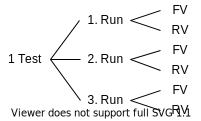
\includegraphics[]{runs}
\end{figure}

For one test, we have actually six times that the website gets loaded and tested.
For e.g. 500 URLs in the bulk test list, we have a total of $500 \times 6 = 3000$ page hits.


\paragraph{Configuration 1}

\begin{table}[h]
	\caption[Test Runs]{Configuration 1}
	\label{tab:tamodelleVergleich}
	\centering
	\begin{tabular}{ |c|c| } 
	\hline
	Configuration Setting & Option \\
	\hline
	Test Location & Test Location \\ 
	Browser & Chrome \\
	\hline
	Connection & LAN \\
	Number of Tests to Run & 3 \\
	Repeat View & First View and Repeat View \\
	Capture Video & True \\
	Keep Test Private & False \\
	Label & none \\
	\hline	  
	Advanced Tab & Nothing selected \\
	Chromium Tab & Nothing selected  \\
	Auth, Script, Block, SPOF, Custom Tabs & Nothing  \\
	Bulk Testing Tab & URL aramyesildeniz... 100 times \\
	\hline
	\end{tabular}
\end{table}

\paragraph{Configuration 2}

Emulate Mobile Browser



\subsubsection{Traffic Shaping}

\begin{itemize}
\item Important to have stable and realistic network condition
\item Chromes tool is not the best for this % see blogpost https://calendar.perfplanet.com/2016/testing-with-realistic-networking-conditions/
\item Private WPT Instance docker on mac does not allow traffic shaping functionality from WPT
\item I use Network Link Conditioner from Apple to slow down the whole machine. See in same blogpost that Patrick highly recommends this
\item WPT also slows down their whole machines % https://forums.webpagetest.org/t/measure-internet-speed/11593
\item IN general internet connection is very unstable. If i run network link conditionier with e.g. DSL each speedtest gives different results. And other test platforms such as fast.com gives also different result.
\end{itemize}





% --------------------------------------------------------



\subsection{Website Variations}

Positions:
1: Top of head element
2: just before closing head element
3: just before closing body element

\begin{center}
	\begin{longtable}{ |c|c|c|c|  }
	\hline
	Variant & Attribute & Position & Additional Scripts \\
	  \hline
	  \rowcolor{lightgrey}
	   Variant 1 & none & 1 & no \\
	  \rowcolor{lightgrey}
	  Variant 3 & async & 1 & no \\
	   & defer & 1 & no \\
	   
  	   & none & 2 & no \\
	   & async & 2 & no \\
  	   & defer & 2 & no \\

  	   & none & 3 & no \\
	   & async & 3 & no \\
  	   & defer & 3 & no \\
  	   
	  \rowcolor{lightgrey}
	   Variant 2 & none & 1 & yes \\
	   & async & 1 & yes \\
  	   & defer & 1 & yes \\

  	   & none & 2 & yes \\
	   & async & 2 & yes \\
  	   & defer & 2 & yes \\

  	   & none & 3 & yes \\
	   & async & 3 & yes \\
  	   & defer & 3 & yes \\
	  \hline
	\caption{Your caption here} % needs to go inside longtable environment
	\label{tab:myfirstlongtable}
	\end{longtable}
\end{center}



\paragraph{variant1.html}


\paragraph{variant2.html}



\paragraph{variant3.html}



% --------------------------------------------------------


\subsection{Test Plan}

The Google Analytics code is more or less fixed and there are no configurations.
It would be possible to change config of script, e.g. change sample rate, track other metrics etc.
But it is not possible to change default tracking behaviour (?)

How the script is included into the file should reflected withing Website Variations

% add Date as column? e.g. 2021-03-25
\begin{table}[h]
	\caption[Test Runs]{Test Runs \cite{DBLP:books/infix/Schwarz99}}
	\label{tab:tamodelleVergleich}
	\centering
	\begin{tabular}{ |c|c|c } 
	 \hline
	  WPT & Website & Date \\
	  \hline
	  C1 & V1 & 2021-04-01 \\ 
	  .. & .. & ..\\ 
	  \hline
	  \end{tabular}
\end{table}




% --------------------------------------------------------




\subsection{Tool support for diagrams and data analysis}

\begin{itemize}
\item python
\item Matplotlib
\end{itemize}


\chapter{Evaluation}


\includegraphics[width=1\textwidth]{test}


\begin{itemize}
	\item Last chapter...
	\item This chapter: Describe shortly all sections from this chapter
	\item In the next chapter...
\end{itemize}





% ----------------------------------------------------------------------------------------------------
% ----------------------------------------------------------------------------------------------------


\section{Test Results}

\subsection{Metrics for Evaluation}

Page Weight: Measured by WPT:
- bytes
- bytes uncompressed
- Requests


Technical Timings / API: Measured by WPT and GA:
- page load time
- domain lookup time
- page download time
- redirection time
- server connection time
- server response time
- Dom interactive time
- Dom content loaded time

Visual Metrics / Web Vitals: Measured by WPT
TODO Measure also with GA / own script ??:
- CLS
- FCP
- FMP
- LCP
- SI

- Visually complete ?
- Time  to Interactive ? Is this the same as DOM interactive time ?

Core Web Vital FID ?? -> Can not be measured without real users...

From WPT bulk section. Also include this somewhere for comparison ?:
- Filmstrips ?
- Waterfall ?
- Visual Progress ?
- Layout Shifts ?



\subsection{Original vs Mock Plain}



\subsection{Mock Plain vs Position 1 (which is default position of GA: Check this again!)}
TODO rename this like with GA true false ?



\subsection{Position 1 vs 2 vs 3}



\subsection{Attribute 1 vs 2 vs 3}



\subsection{Other script True vs False}







% ----------------------------------------------------------------------------------------------------
% ----------------------------------------------------------------------------------------------------


\section{General}

\begin{itemize}
    \item For each attempt, describe: Threats to validity, generalizability
\end{itemize}

generalizability: meine Daten zeige nur für Chrome, MacBook, diese Geschwindigkeit etc.
Und auch nur für diese Test-Website
Die Schwierigkeit der Generalisierbarkeit ist eines der grössten Probleme bei dieser Fragestellung


% TODO get rid of this? Maybe just evaluate all other apporaches quickly in approach section?

\section{Plain / Skeletal Website}

\begin{itemize}
\item Information gained from this experiment
\item Limitations and questions which can not be answered with this approach
\end{itemize}


\section{Mirroring}


\section{HTTP Archive inspired website}

\begin{itemize}
\item Information gained from this experiment
\item Meaning and interpretation of the collected data
\item Limitations and questions which can not be answered with this approach
\end{itemize}





% TODO rework sections below. Here i dont need to present all options / results from WPT again but rather my results ??

\section{WebPageTest Bulk Tests}

\begin{itemize}
\item Bulk testing is a feature for private instances only
\item Misuse this feature to test the same website X times
\end{itemize}


\subsection{Bulk Test Overview: Description of test result page}

\begin{itemize}
\item Each test has Test ID: YYMMDD\textunderscore random\textunderscore random
\item Test results after bulk test available under \url{http://localhost:4000/result/{testID}/}
\item For each test run, following data is available:
	\begin{itemize}
	\item Link to test results: Test result page as same as for single test run
	\item Median load time (First view)
	\item Median load time (Repeat view)
	\item Median Speed Index (First View)
	\item Raw page data (file: [TestID\textunderscore summary.csv]
	\item Raw object data (file: [TestID\textunderscore details.csv])
	\item Http archive (.har) (file: json)
	\end{itemize}
	
\item Average First View Load Time
\item Average Repeat View Load Time
\item Combined Raw: Page Data  (file: [TestID\textunderscore summary.csv])
\item Combined Raw: Object Data (file: [TestID\textunderscore details.csv]). For 100 test runs, this file is appr. 20 MB, 24432 rows, 76 columns. 
\item Aggregate Statistics (file: [TestID\textunderscore aggregate.csv])
\end{itemize}


\subsection{Summary File for one Test}

\begin{itemize}
\item Contains 6 rows: 3 test runs: for each test runs 1x first view and 1x repeat view
\item Rows 1, 3, 5 contain FV, rows 2, 4, 6 contain data for RV
\end{itemize}

\subsection{Aggregate Statistics File}

\begin{itemize}
\item Contains aggregated data from bulk test
\item One row for each test run: For 100 URLs in bulk test will be 100 rows in csv
\item Each metric is available with Median, Average, Standard Deviation, Min, Max
\item Metrics are available once from FV and once for Repeat View
\item Metrics:
	\begin{itemize}
	\item Successful Tests
	\item Document Complete
	\item Fully Loaded
	\item First Byte
	\item Start Render
	\item Bytes In (Doc)
	\item Requests (Doc)
	\item Load Event Start
	\item Speed Index
	\item Last Visual Change
	\item Visually Complete
	\end{itemize}
\item => For metric details, see Terms and Definitions
\end{itemize}


\subsection{Compare Section}

WPT has a feature to compare multiple tests.
Accessible under compare URL: \url{http://localhost:4000/video/compare.php?tests={TestID},{TestID},...}

The compare page contains:

\begin{itemize}
\item Film strip
\item Waterfall diagram
\item Visual Progress diagram
\item Timings diagram:
	\begin{itemize}
	\item Visually Complete (First View Visually Complete Median)
	\item Last Visual Change
	\item Load Time (onload)
	\item ...
	\end{itemize}
\item Cumulative Layout Shift diagram
\item Requests diagram
\item Bytes diagram
\item Visually complete
\item Last Visual Change
\item Load Time (onload)
\item Load Time (Fully Loaded)
\item DOM Content Loaded
\item Speed Index
\item Time to First Byte
\item Time to Title
\item Time to Start Render
\item CPU Busy Time
\item 85\% Visually Complete
\item 90\% Visually Complete
\item 95\% Visually Complete
\item 99\% Visually Complete
\item First Contentful Paint
\item First Meaningful Paint
\item Largest Contenful Paint
\item Cumulative Layout Shift
\item html Requests
\item html Bytes
\item js Requests
\item js Bytes
\item css Requests
\item css Bytes
\item image Requests
\item image Bytes
\item flash Requests
\item flash Bytes
\item font Requests
\item font Bytes
\item video Requests
\item video Bytes
\item other Requests
\item other Bytes
\end{itemize}







\section{Internal, external validity}


\begin{itemize}
\item At this point, i have the data collected and can analyse it
\item The quality and quantity of the data needs to be discussed
\item Quality: There are chances that some data are malformed, e.g. because internet connection was bad, etc.
\item Quantity: Is the amount of data sufficient to make the evaluation generalisable
\end{itemize}


% 2016 Kohavi: Analysis of Experiments


\chapter{Future Work}

\begin{itemize}
	\item Last chapter...
	\item This chapter: Describe shortly all sections from this chapter
	\item In the next chapter...
\end{itemize}

\section{Limitations of this thesis}

\begin{itemize}
\item Discussion of unobserved topics
\item Discussion of possible next steps
\end{itemize}

\section{Other measurement tools and metrics}

\begin{itemize}
\item List of tools and metrics worth investigating
\end{itemize}

\subsection{Google Analytics 4}


\section{Speed Kit}

% 2020 Wolle


\section{PWAs, AMPs, Service Workers, Caching, HTTP2 etc.}

\begin{itemize}
\item Overview of other web technologies and how they could be relevant for further research
\end{itemize}

% Test for Mobile users:
% Mobile shopping on the rise: https://einzelhandel.de/presse/zahlenfaktengrafiken/861-online-handel/4761-bedeutung-der-smartphones-im-onlinehandel
% They are generally more unhappy: https://einzelhandel.de/presse/zahlenfaktengrafiken/861-online-handel/4462-mobile-optimierung-online-shop

% Not covered: Beaconing aspect: When to send data back home, at which time is best, what is tradeoff etc.

% Create a user journey with a script for WPT

\chapter{Conclusion}

\begin{itemize}
	\item Last chapter...
	\item This chapter: Describe shortly all sections from this chapter
\end{itemize}

\begin{itemize}
\item Scope and contribution of this thesis
\item Short summary of each chapter:
	\begin{itemize}
	\item Problem statement and why it is worth to examine research question
	\item Terms and definitions
	\item (Related work)
	\item Approach and evaluation of practical work
	\item Future work
	\end{itemize}
\end{itemize}

\chapter{Appendix}

\section{Test Object Variants}


\subsection{IV Position}

\begin{sidewaysfigure}
\begin{multicols}{3}
\begin{center}
\begin{lstlisting}[caption={Position 1}, language=html, numbers=none]
<!DOCTYPE html>
<html>
    <head>
        <!-- Google Analytics -->
        <script></script>
        <!-- End Google Analytics -->

        <title>
        <meta>
        <link>
        <script>
    </head>

    <body>
        ...
    </body>
</html>
\end{lstlisting}
\end{center}

\columnbreak

\begin{center}
\begin{lstlisting}[caption={Position 2}, language=html, numbers=none]
<!DOCTYPE html>
<html>
    <head>
        <title>
        <meta>
        <link>
        <script>
        
        <!-- Google Analytics -->
        <script></script>
        <!-- End Google Analytics -->
    </head>

    <body>
        ...
    </body>
</html>
\end{lstlisting}
\end{center}

\columnbreak

\begin{center}
\begin{lstlisting}[caption={Position 3}, language=html, numbers=none]
<!DOCTYPE html>
<html>
    <head>
        <title>
        <meta>
        <link>
        <script>
        
    </head>

    <body>
        ...
        <!-- Google Analytics -->
        <script></script>
        <!-- End Google Analytics -->
    </body>
</html>
\end{lstlisting}
\end{center}
\end{multicols}
\end{sidewaysfigure}


\subsection{IV 2 Attribute}

\begin{sidewaysfigure}
\begin{multicols}{3}
\begin{center}
\begin{lstlisting}[caption={Attribute 1}, language=html, numbers=none]
<!DOCTYPE html>
<html>
    <head>
        <!-- Google Analytics -->
        <script></script>
        <!-- End Google Analytics -->

        <title>
        <meta>
        <link>
        <script>
    </head>

    <body>
        ...
    </body>
</html>
\end{lstlisting}
\end{center}

\columnbreak

\begin{center}
\begin{lstlisting}[caption={Attribute 2}, language=html, numbers=none]
<!DOCTYPE html>
<html>
    <head>
        <!-- Google Analytics -->
        <script async></script>
        <!-- End Google Analytics -->

        <title>
        <meta>
        <link>
        <script>
    </head>

    <body>
        ...
    </body>
</html>
\end{lstlisting}
\end{center}

\columnbreak

\begin{center}
\begin{lstlisting}[caption={Attribute 3}, language=html, numbers=none]
<!DOCTYPE html>
<html>
    <head>
        <!-- Google Analytics -->
        <script defer></script>
        <!-- End Google Analytics -->

        <title>
        <meta>
        <link>
        <script>
    </head>

    <body>
        ...
    </body>
</html>
\end{lstlisting}
\end{center}
\end{multicols}
\end{sidewaysfigure}








\subsection{IV 3 Other Script}

\begin{sidewaysfigure}
\begin{multicols}{2}
\begin{center}
\begin{lstlisting}[caption={Other Script 1}, language=html, numbers=none]
<!DOCTYPE html>
<html>
    <head>
        <!-- Google Analytics -->
        <script></script>
        <!-- End Google Analytics -->
        




        <title>
        <meta>
        <link>
        <script>
    </head>

    <body>
        ...
    </body>
</html>
\end{lstlisting}
\end{center}

\columnbreak

\begin{center}
\begin{lstlisting}[caption={Other Script 2}, language=html, numbers=none]
<!DOCTYPE html>
<html>
    <head>
        <!-- Google Analytics -->
        <script></script>
        <!-- End Google Analytics -->
        
        <!-- Other Script-->
        <script></script>
        <!-- End Other Script -->

        <title>
        <meta>
        <link>
        <script>
    </head>

    <body>
        ...
    </body>
</html>
\end{lstlisting}
\end{center}
\end{multicols}
\end{sidewaysfigure}


% ------------------------------------------------------------------------------------------------



\subsection{Single Test Raw page data}

WPT Metrics from summary file
\begin{center}
	\small
	\begin{longtable}{ p{0.4\linewidth} | p{0.6\linewidth} }
	Name & Description \\ 
	\hline
        minify\textunderscore total & Total bytes of minifiable text static assets. \\
        responses\textunderscore 200 & The number of responses with HTTP status code of 200, OK. \\
        testStartOffset & ... \\
        bytesOut & The total bytes sent from the browser to other servers. \\
        gzip\textunderscore savings & Total bytes of compressed responses. \\
        requestsFull & ... \\
        start\textunderscore epoch & ... \\
        connections & The number of connections used. \\
        base\textunderscore page\textunderscore cdn & The CDN provider for the base page. \\
        bytesOutDoc & Same as bytesOut but only includes bytes until the Document Complete
event. Usually when all the page content has loaded (window.onload). \\
        result & Test result code. \\
        final\textunderscore base\textunderscore page\textunderscore request\textunderscore id & ... \\
        basePageSSLTime & ... \\
        docTime & Same as loadTime. \\
        domContentLoadedEventEnd & Time in ms since navigation started until document DOMContentLoaded event finished. \\
        image\textunderscore savings & Total bytes of compressed images. \\
        requestsDoc & The number of requests until Document Complete event. \\
        firstMeaningfulPaint & ... \\
        score\textunderscore cookies & WebPageTest performance review score for not using cookies on static assets. \\
        firstPaint & RUM First Paint Time, the time in ms when browser first painted something on screen. It's calculated on the client for browsers that implement this method. \\
        score\textunderscore cdn & WebPageTest performance review score for using CDN for all static assets. \\
        optimization\textunderscore checked & Whether or not optmizations were checked. \\
        score\textunderscore minify & WebPageTest performance review score for minifying text static assets. \\
        gzip\textunderscore total & Total bytes of compressible responses. \\
        responses\textunderscore 404 & The number of responses with HTTP status code of 404, not found. \\
        loadTime & The total time taken to load the page (window.onload) in ms. \\
        URL & The tested page URL. \\
        score\textunderscore combine & WebPageTest performance review score for bundling JavaScript
and/or CSS assets. \\
        firstContentfulPaint & ... \\
        image\textunderscore total & Total bytes of images. \\
        score\textunderscore etags & WebPageTest performance review score for disabling *ETag*s. \\
        loadEventStart & Time in ms since navigation started until window.onload event was triggered (from W3C Navigation Timing). \\
        minify\textunderscore savings & Total bytes of minified text static assets. \\
        score\textunderscore progressive\textunderscore jpeg & WebPageTest performance review score for using progressive JPEG. \\
        domInteractive & ... \\
        score\textunderscore gzip & WebPageTest performance review score for using gzip compression for
transferring compressable responses. \\
        score\textunderscore compress & WebPageTest performance review score for compressing images. \\
        domContentLoadedEventStart & Time in ms since navigation started until document DOMContentLoaded event was triggered (from W3C Navigation Timing). \\
        final\textunderscore url & ... \\
        bytesInDoc & Same as bytestIn but only includes bytes until Document Complete event. \\
        firstImagePaint & ... \\
        score\textunderscore keep-alive & WebPageTest performance review score for using persistent connections. \\
        loadEventEnd & Time in ms since navigation started until window.onload event finished. \\
        cached &  0 for first view or 1 for repeat view. \\
        score\textunderscore cache & WebPageTest performance review score for leveraging browser caching of static assets. \\
        responses\textunderscore other & The number of responses with HTTPS status code different from 200 or 404. \\
        main\textunderscore frame & ... \\
        fullyLoaded & The time (in ms) the page took to be fully loaded — e.g., 2 seconds of no network activity after Document Complete. This will usually include any activity that is triggered by javascript after the main page loads. \\
        requests & List of details of all requests on tested page. \\
        final\textunderscore base\textunderscore page\textunderscore request & ... \\
        TTFB & Time to first byte, which is the duration in ms from when the user first made the HTTP request to the very first byte of the page being received by the browser. \\
        bytesIn & The amount of data that browser had to download in order to load the page. It
is also commonly referred to as the page size. \\
        osPlatform & ... \\
        test\textunderscore run\textunderscore time\textunderscore ms & ... \\
        tester & The ID of tester that performed the page test. \\
        browser\textunderscore version & The browser version. \\
        document\textunderscore origin & ... \\
        document\textunderscore URL & ... \\
        date & Time and date (number of seconds since Epoch) when test was complete. \\
        PerformancePaintTiming.first-paint & ... \\
        osVersion & ... \\
        domElements & The total number of DOM elements. \\
        browserVersion & The browser version. \\
        fullyLoadedCPUms & CPU busy time in ms until page was fully loaded. \\
        browser\textunderscore name & The browser name. \\
        PerformancePaintTiming.first-contentful-paint & ... \\
        base\textunderscore page\textunderscore cname & ... \\
        eventName & ... \\
        os\textunderscore version & ... \\
        base\textunderscore page\textunderscore dns\textunderscore server & ... \\
        fullyLoadedCPUpct & Average CPU utilization up until page is fully loaded. \\
        domComplete & ... \\
        base\textunderscore page\textunderscore ip\textunderscore ptr & ... \\
        document\textunderscore hostname & ... \\
        lastVisualChange & Time in ms until the last visual changed occured. \\
        visualComplete & Time in ms when page was visually completed. \\
        render & The first point in time (in ms) that something was displayed to the screen. Before that user was staring at a blank page. This does not necessarily mean the user saw the page content — it could just be something as simple as a background color — but it is the first indication of something happening for the user. \\
        SpeedIndex & The SpeedIndex score. \\
        visualComplete85 & Time in ms when page was visually completed 85\%. \\
        visualComplete90 & Time in ms when page was visually completed 90\%. \\
        visualComplete95 & Time in ms when page was visually completed 95\%. \\
        visualComplete99 & Time in ms when page was visually completed 99\%. \\
        LargestContentfulPaintType & ... \\
        LargestContentfulPaintNodeType & ... \\
        chromeUserTiming.navigationStart & ... \\
        chromeUserTiming.fetchStart & ... \\
        chromeUserTiming.responseEnd & ... \\
        chromeUserTiming.domLoading & ... \\
        chromeUserTiming.markAsMainFrame & ... \\
        chromeUserTiming.domInteractive & ... \\
        chromeUserTiming.domContentLoadedEventStart & ... \\
        chromeUserTiming.domContentLoadedEventEnd & ... \\
        chromeUserTiming.firstPaint & ... \\
        chromeUserTiming.firstContentfulPaint & ... \\
        chromeUserTiming.firstImagePaint & ... \\
        chromeUserTiming.firstMeaningfulPaint & ... \\
        chromeUserTiming.firstMeaningfulPaintCandidate & ... \\
        chromeUserTiming.domComplete & ... \\
        chromeUserTiming.loadEventStart & ... \\
        chromeUserTiming.loadEventEnd & ... \\
        chromeUserTiming.LargestContentfulPaint & ... \\
        chromeUserTiming.LargestTextPaint & ... \\
        chromeUserTiming.CumulativeLayoutShift & ... \\
        run & The run number. \\
        step & ... \\
        effectiveBps & Bytes per seconds, i.e.: total of bytes in / total time to load the page. \\
        effectiveBpsDoc & Same as effectiveBps but until Document Complete event. \\
        domTime & The total time in ms until a given DOM element (specified via domelement parameter when running a test) was found on the page. \\
        aft & Above the Fold Time (no longer supported). The time taken to load everything in
the viewport above the fold. \\
        titleTime & Total time in ms until page title was set on browser. \\
        domLoading & ... \\
        server\textunderscore rtt & ... \\
        smallImageCount & ... \\
        bigImageCount & ... \\
        maybeCaptcha & ... \\
        bytes.html & ... \\
        requests.html & ... \\
        bytesUncompressed.html & ... \\
        bytes.js & ... \\
        requests.js & ... \\
        bytesUncompressed.js & ... \\
        bytes.css & ... \\
        requests.css & ... \\
        bytesUncompressed.css & ... \\
        bytes.image & ... \\
        requests.image & ... \\
        bytesUncompressed.image & ... \\
        bytes.flash & ... \\
        requests.flash & ... \\
        bytesUncompressed.flash & ... \\
        bytes.font & ... \\
        requests.font & ... \\
        bytesUncompressed.font & ... \\
        bytes.video & ... \\
        requests.video & ... \\
        bytesUncompressed.video & ... \\
        bytes.other & ... \\
        requests.other & ... \\
        bytesUncompressed.other & ... \\
        id & ... \\
        chromeUserTiming.InteractiveTime & ... \\
     \caption{Your caption here} % needs to go inside longtable environment
	\label{tab:myfirstlongtable}
	\end{longtable}
\end{center}



\cleardoublepage



% VERZEICHNISSE (Abbildungen, Tabellen)
% Literatur
\nocite{wiki:wissarbeit}
\bibliographystyle{alphadin}
\bibliography{thesis}
\cleardoublepage




% ERKLÄRUNG
\input{_eidversicherung}



    
\end{document}